%% Mẫu luận án tiến sĩ (thạc sĩ) theo style vietkey.luanan.1.2.cls - Version 1.2
%% (c) Dang Minh Tuan, Vietkey Group.
%% Tel: +84-98-868-6636, Email: tuanvietkey@gmail.com.
%%
%% History:
%% - version 1.2 (2017/08/11)
%% - Created on 2016/08/16.

\documentclass[fontsize=13pt,twoside,a4paper,openright]{vietkey.luanan.1.2}

%tham số firstinits=true để viết tắt, defernumbers để số thứ tự liền mạch.
\usepackage[backend=bibtex,
            bibstyle=luanan,
            % style=ieee,
            sorting=none,
            block=none,
            %defernumbers=true,
            babel=other]{biblatex}
\usepackage{titling}
\usepackage{setspace}
\usepackage{fancyvrb}
\usepackage{dirtytalk}
\usepackage{listing}
\usepackage{listings-rust}
\usepackage[acronym]{glossaries}


\lstdefinelanguage{windbg}{
      % backgroundcolor=\color{black!10},
      % basicstyle=\footnotesize \ttfamily \color{black} \bfseries,
      breakatwhitespace=false,
      breaklines=false,
      captionpos=t,
      % commentstyle=\color{dkgreen},
      deletekeywords={...},
      escapeinside={\%*}{*)},
      frame=tb,
      keywordstyle=\color{purple},
      morekeywords={kd,dt,Ptr64,Void,UChar,Uint4B,Uint8B,Int4B,Int2B,long,void},
      identifierstyle=\color{black},
      stringstyle=\color{blue},
      numbers=left,
      numbersep=5pt,
      numberstyle=\tiny\color{black},
      rulecolor=\color{black},
      showspaces=false,
      showstringspaces=false,
      showtabs=false,
      stepnumber=1,
      tabsize=4,
      basicstyle=\linespread{1}\tiny\ttfamily,
      title=\lstname,
}

\lstdefinelanguage{cpp}{
      % backgroundcolor=\color{black!10},
      % basicstyle=\footnotesize \ttfamily \color{black} \bfseries,
      breakatwhitespace=false,
      breaklines=false,
      captionpos=t,
      % commentstyle=\color{dkgreen},
      deletekeywords={...},
      escapeinside={\%*}{*)},
      frame=tb,
      language=C++,
      keywordstyle=\color{purple},
      morekeywords={NTSTATUS,HANDLE,PEPROCESS},
      identifierstyle=\color{black},
      stringstyle=\color{blue},
      numbers=left,
      numbersep=5pt,
      numberstyle=\tiny\color{black},
      rulecolor=\color{black},
      showspaces=false,
      showstringspaces=false,
      showtabs=false,
      stepnumber=1,
      tabsize=4,
      basicstyle=\linespread{1}\tiny\ttfamily,
      title=\lstname,
}

% Use hyphens PassOptions to add hyphenation in long urls
% \PassOptionsToPackage{hyphens}{url}\usepackage[unicode]{hyperref}

% Do not use these two following settings, which cause weird paragraph spacing
% \widowpenalty=1000 % remove widow lines
% \clubpenalty=1000 % remove orphan lines

\hyphenpenalty 10000
% \exhyphenpenalty 10000

\DeclareCaptionFormat{listing}{\rule{\dimexpr\textwidth+1pt\relax}{0.1pt}\vspace{-6pt}\par#1#2#3}
\captionsetup[lstlisting]{format=listing,singlelinecheck=false, margin=0pt, font={sf},labelsep=space,labelfont=bf}

\addbibresource{../bibdmt.bib}                 %%% dữ liệu về tài liệu tham khảo.
\begin{document}

% ==================== PAGE ORDERING =================
% Title Page
% Copyright Page
% Abstract
% Dedication, Acknowledgements, and Preface (each optional)
% Table of Contents, with page numbers
% List of Tables, List of Figures, or List of Illustrations, with titles and page numbers (if applicable)
% List of Abbreviations (if applicable)
% List of Symbols (if applicable)
% Chapters, including:
% Introduction, if any
% Main body, with consistent subheadings as appropriate
% Appendices (if applicable)
% Endnotes (if applicable)
% References (see section on References for options)

\begin{titlingpage}
\begin{singlespace}
% \calccentering{\unitlength}
% \begin{adjustwidth*}{\unitlength}{-\unitlength}

\begin{center}
{\Large \textsc{Vietnam National University \\Ho Chi Minh city University of Techonology}\\
\vspace{3mm}
Faculty of Computer Science and Engineering
}\\
\vspace{10mm}
% \vspace*{13mm}
\includegraphics[width=0.3\textwidth]{images/logo.png}\\
\vspace{1cm}
\rule[0.5ex]{\linewidth}{2pt}\vspace*{-\baselineskip}\vspace*{3.2pt}
\rule[0.5ex]{\linewidth}{1pt}\\[\baselineskip]
{\huge \textcolor{blue}{Windows Memory Forensics}}\\[4mm]
{\Large \textit{\textcolor{blue}{Finding hidden processes in a running machine}}}\\
\rule[0.5ex]{\linewidth}{1pt}\vspace*{-\baselineskip}\vspace{3.2pt}
\rule[0.5ex]{\linewidth}{2pt}\\
\vspace{6.5mm}
{\large By}\\
\vspace{6.5mm}
{\Large\textsc{NGUYEN Anh Khoa - 1611617}}\\
{\Large\textsc{\textbf{Major}: Computer Science}}\\
\vspace{12mm}

\begin{minipage}{12cm}
A dissertation submitted to the University of Technology, VNU-HCM in accordance with the requirements of the DEGREE OF ENGINEER in Computer Science.
\end{minipage}\\

\vspace{6mm}
\begin{center}
\begin{tabular}{ r l }
\textbf{Instructors}:& \Large \textsc{Dr. NGUYEN An Khuong}\\
& \Large \textsc{Mr. NGUYEN Le Thanh}\\
& \Large \textsc{Mr. NGUYEN Quoc Bao}\\
\textbf{Opponent}:& \Large \textsc{Dr. TRAN Tuan Anh}\\
\end{tabular}
\end{center}
\vspace{7mm}
{\large Ho Chi Minh City, \textsc{July 2020}}
\end{center}
% \end{adjustwidth*}
\end{singlespace}
\end{titlingpage}
                          %%% có thể thay đổi
% \include{loicamdoan}                        %%% có thể thay đổi
% \include{loicamon}                          %%% có thể thay đổi
\input{abstract.tex}
\VKnumRoman                                 %%% đánh số bằng chữ cái i, ii...
\blankpage
\VKmucLuc                                   %%% mục lục
% \include{kyhieu}                            %%% có thể thay đổi
\VKdanhMucHinhVe                            %%% danh mục hình vẽ
\VKdanhMucBangBieu                          %%% danh mục bảng biểu
%\VKdanhMucDinhLy
%\VKdanhMucDinhNghia
\VKdanhMucListings
\input{glossary.tex}
\VKbatDaudanhSo                             %%% bắt đầu đánh số từ 1,2,3...
\blankpage
% \include{loinoidau}                         %%% có thể thay đổi

\chapter[Introduction]{Introduction}

\section[Motivation]{Motivation}

Through computer development, computers have become a standard method for
humans around the world to study, work, and entertain. Most activities of our
daily lives involve computers. Individuals across the globe have created
systems running on computers to assist them in doing from trivial to complex
tasks. However, this somehow influenced other people to commit harmful
activities, and these people are often referred to as \textit{hacker}.  Hackers
have been creating software causing damage and steal confidential or private
information, and these types of software are malware. In the early days of
malware, they are often harmless, created to disturb the owner of the infected
machine.  Then soon, they became severe threats, breaking the systems, stealing
data, asking for ransom. The battle between malware writers and malware
analysts has started, since 1971, and no sign of stopping.

Malware analysts have been struggling to protect the system from malware.
However, it has never come close to perfection. The most efficient resolution
to the problem uses file checksum with unique bytes sequences in a particular
malware to form the malware's signature. A list of malware's signature, for
example, Yara rules \cite{yararules}, is then checked for every file upon
entering the system, whether it is file downloading or copying from USB to
disk. Relying on malware's signature for filtering files often miss out newer
ones. Thus, it is highly vulnerable to the newer class of malware. When the
system is infected with unknown malware, malware analysts perform digital
forensics to capture the malware and learn about its behavior. Digital
forensics, as described in A Road Map for Digital Forensic Research
\cite{roadmap}:


\say{The use of scientifically derived and proven methods toward the
preservation, collection, validation, identification, analysis, interpretation,
documentation and presentation of digital evidence derived from digital sources
for the purpose of facilitating or furthering the reconstruction of events
found to be criminal, or helping to anticipate unauthorized actions shown to be
disruptive to planned operations.}

Digital forensics includes many different aspects, while the most intrigued
part of digital forensics is memory forensics. Memory forensics ``provides
unprecedented visibility into the runtime state of the system, such as which
processes were running, open network connections, and recently executed
commands,'' as stated in the book The Art of Memory Forensics
\cite{ligh2014art}. By doing memory forensics, we can collect evidence and
reveal what causes the system to misbehave and malware behavior.  Digital
forensics happens after a malware is found in the system, but what if it has
never been found. In cases where it was disguising as legitimate software, or
it was hiding from the system. In these scenarios, we fail to detect and
perform any analysis.

From the early days of the 1990s, malware writers have been improving ways to
hide the malware. In 2017, a small report \cite{evolutionHidding} has revised
on hiding techniques used by malware over the years in the Windows OS. Most of
these techniques are either preventable or mitigable. However, even in 2019,
one can still observe incidences where malware hides so effectively. For
example, the \textit{Titanium} backdoor\footnote{Programs that receives remote
connections} on Windows 10 disclosed November 2019 \cite{titanium}. These
incidences are reported by experts who are experienced in digital forensics and
malware analysis. We tried to find a solution where a simple program can
perform digital forensics and report the current machine status. Many solutions
came up, but they do not work out-of-the-box, the user must install Python (at
least), extract the memory, and then perform forensics on the memory file, all
too troublesome. We turn our research into doing forensics on a running system,
live forensics, but it has limited research, although feasible
\cite{reviewLive}. As a result of this, we propose a quick and nice solution to
do live forensics on the Windows machine that removes the troublesome. The
outcome of the solution is a small CLI tooling capable of doing forensics on
multiple Windows versions.

\section[Thesis outcome]{Thesis outcome}

This thesis outcome is a small program demonstrating live forensics ability
without memory acquisition. We try to apply with the current forensics
technique to find hidden malware with the tool. As a result, we expect our tool
to implement these techniques. These techniques will be discussed later in
Chapter 3.

\begin{itemize}
  \item Traverse some important system lists
  \item Pool tag scanning
  \item SSDT table and IRP inspection
  \item Show unloaded drivers
\end{itemize}

With the above features, this thesis should reach these goals:

\begin{itemize}
% \setlength\itemsep{-0.5em}
  \item Understand the basics concept of OS that supports memory forensics,
  \item Understand to some extent of Windows internals,
  \item Understand some techniques often used to do Windows memory forensics,
  \item Analyze some already existed tools doing memory forensics,
  \item Implement the tool to find hidden malware.
\end{itemize}

\section[Structure]{Structure}

\begin{itemize}
  \item Chapter 1 gives an overview, the goals and challenges of this thesis proposal,
  \item Chapter 2 presents the background on OS, Windows Internal and malware prevention technology,
  \item Chapter 3 introduces malware hiding techniques and ways to find them using forensics methods,
  \item Chapter 4 reviews some related works,
  \item Chapter 5 lists the tools used when developing,
  \item Chapter 6 suggests our solution,
  \item Chapter 7 discusses on the solution's applications and their results,
  \item Chapter 8 disputes about the strengths and limitation in our solution,
  \item Chapter 9 concludes our thesis.
\end{itemize}

\chapter[Background]{Background}

This thesis is built up using many backgrounds on memory management, the
Windows internals and some malware prevention technology. This chapter will
give readers a quick summary to understand these key points. The chapter
heavily depends on these materials \cite{ligh2014art}
\cite{russinovich2012windows}.

\section[Fundamental OS]{Fundamental OS}

Understanding how the operating system works is fundamental when developing a
forensics tools. In this thesis, the OS memory management is a required
knowledge. Which is why in this section, we will go through these OS concepts,
pagination, virtual memory, and the OS kernel.

\subsection[Pagination]{Pagination}

Pagination, or paging, is a memory management scheme used by many modern
operating systems. In this scheme, the operating system handles memory by
blocks of constant size. A block of constant size is called a \textit{page}.
The operating system considers a process as a list of pages when using pagination,
and the physical memory RAM (random-access-memory) as a page holder. When
starting a process, the OS will not load the whole process in RAM but only
loads pages that need to be run. When a page in RAM is no longer needed, it
will be removed, \textit{page out}, and replaced by a higher priority page.
The convention \textit{in memory} states that the page is inside RAM, and a
page not inside RAM is said to be \textit{is disk}. In Figure
\ref{fig:pagination} we can see the OS loads some pages of the process in
memory, and the other pages are in disk.

\begin{figure}[h]
  \centering
  \caption{Pagination}
  \label{fig:pagination}
  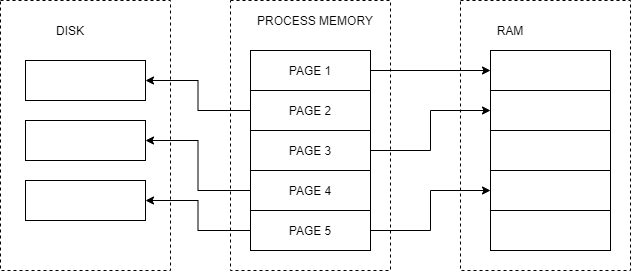
\includegraphics[scale=0.7]{images/pagination.png}
\end{figure}

\subsection[Virtual memory]{Virtual memory}

Virtual memory is a memory management technique where the OS gives an
abstraction level over the addresses indexable by a process. The OS creates a
different address mapping schema for every process running; in other words, two
processes both access the same address results in a different address in RAM.
It is illustrated in Figure \ref{fig:virtualmem}, the two processes have the
same referencing address 0x4000, but in RAM, their addresses are 0x6000 and
0x9000. The address before conversion to RAM address is called virtual address,
and the RAM address is called physical address.

\begin{figure}[h]
  \centering
  \caption{Virtual memory}
  \label{fig:virtualmem}
  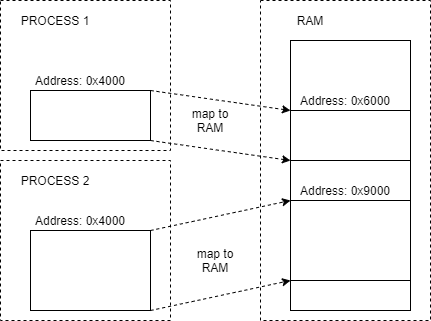
\includegraphics[scale=0.8]{images/virtualmem.png}
\end{figure}

\subsection[Kernel]{Kernel}

The kernel in OS is the program responsible for communicating with the hardware
and controlling other programs. The code for the kernel is loaded in memory
during the machine uptime. The kernel manages critical tasks, including
processes scheduling, memory management, I/O operations.

The kernel handles communication with the hardware through system calls or
\textit{syscall}. There are many implementations to the system call, and the
most common way is by system interrupts.  The kernel will have a syscall table,
which is a table of function pointers. They are called by an interrupt
instruction with the index to the syscall table, as shown in Figure
\ref{fig:syscall}.

\begin{figure}[h]
  \centering
  \caption{System call}
  \label{fig:syscall}
  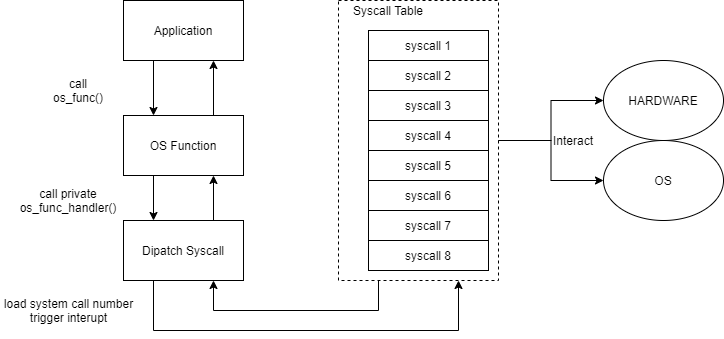
\includegraphics[scale=0.7]{images/syscall.png}
\end{figure}

\subsection[Windows implementation]{Windows implementation}

In Windows 64-bit, pagination is implemented using pages of size 4KB.  Paged
out pages are saved in \texttt{C:\textbackslash\textbackslash Pagefile.sys}.
Virtual memory for every user processes is from 0x0000000000 to 0x7FFFFFFFFFF.
The address from 0x80000000000 to 0xFFFFFFFFFFF is called the system address
space or kernel space.  The system address space is only accessible by the
processes in \textit{kernel-mode}, namely the kernel and kernel drivers.  For
each user process, a separate address space is assigned for the process, but
there is only one system address space and is shared with every kernel
processes running. The user address space and the system address space are
virtual memory, which has to be translated to physical address when access. The
Figure \ref{fig:winimplement} shows the memory layout of the kernel and user
processes memory in Windows 64-bit systems. While the user process can not
access system address space, kernel processes can access any virtual page.

\begin{figure}[h]
  \centering
  \caption{Windows memory layout}
  \label{fig:winimplement}
  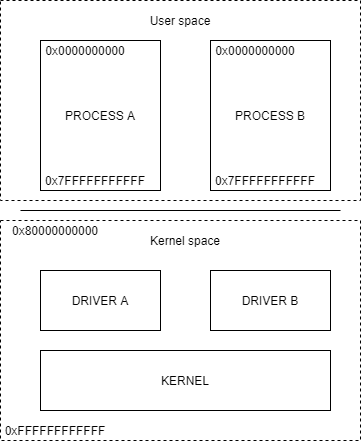
\includegraphics[scale=0.7]{images/winimplement.png}
\end{figure}

Syscall in Windows is called in two ways, and both implemented with a system
call table. The first way is done by interrupting the code 0x2e, and the second
way is using the instruction sysenter/syscall. Both ways receive the index to
the system call table in register edx.

\section[Windows Internal]{Windows Internal}

In this section, we introduce some key points of the Windows operating system.
These key points are executive objects, the kernel pool, the global list, and
debug symbols used by Windows.

\subsection[Executive Objects]{Executive Objects}

Windows executive objects are kernel structures allocated and prepended with
various headers. Only some kernel structures are allocated this way, a common
list of executive objects often used for forensics is in the Table
\ref{tab:execobj}. Executive objects must have a header called
\texttt{\_OBJECT\_HEADER}, but it can have other optional headers data.
Forensics tools often use these headers' data to get some general information
about the allocation. Below we discuss some kernel structures and their roles
in the Windows operating system.

\begin{table}[t]
\centering
\begin{tabular}{ll}
\hline
  Object        & Structure                         \\ \hline
  Process       & \texttt{\_EPROCESS}               \\
  Thread        & \texttt{\_ETHREAD}                \\
  File          & \texttt{\_FILE\_OBJECT}           \\
  Driver        & \texttt{\_DRIVER\_OBJECT}         \\
  Mutex         & \texttt{\_KMUTANT}                \\
  Token         & \texttt{\_TOKEN}                  \\
  Symbolic link & \texttt{\_OBJECT\_SYMBOLIC\_LINK} \\
  Type          & \texttt{\_OBJECT\_TYPE}           \\
  Key           & \texttt{\_CM\_HIVE}               \\
\end{tabular}
\caption{Comprehensive list of executive objects}
\label{tab:execobj}
\end{table}

\subsubsection[EPROCESS]{EPROCESS}

\texttt{\_EPROCESS}, Listing \ref{lst:eprocess}, is a structure to manage the
running process. This structure contains the process id, the parent process id,
the memory map for the process, the process environment block, the pointer to
list of loaded modules, the pointer to list of threads created by the process
and other information related to the process.  This structure is also a node in
a circular doubly linked list of processes.

The memory map is the list of sections inside a process address space, and
these are code, data, heap, libraries. It is represented as a self-balancing
tree where each node contains the address, size, and operations
(Read/Write/Execution) allowed in the region. This tree is often called as
\textit{Vad tree}, and the root of the tree is the \texttt{VadRoot} member in
\texttt{\_EPROCESS}.

The process environment block (PEB), Listing \ref{lst:peb}, contains the
information to the process, such as the image base address, the heap pointer.
This block resides in the user space memory, so the kernel process can not read
this information without mapping the user space into the kernel space. The
pointer to the address of the block is the \texttt{PEB} member of
\texttt{\_EPROCESS} and we can map the page containing the PEB to read the
process information.

\begin{lstlisting}[language=windbg,lable={lst:eprocess},caption=\texttt{\_EPROCESS} in Windows 7,float,floatplacement=H]
kd> dt _EPROCESS
nt!_EPROCESS
   +0x168 CreateTime       : _LARGE_INTEGER
   +0x170 ExitTime         : _LARGE_INTEGER
   +0x180 UniqueProcessId  : Ptr64 Void
   +0x188 ActiveProcessLinks : _LIST_ENTRY
   +0x238 PhysicalVadRoot  : Ptr64 _MM_AVL_TABLE
   +0x258 Win32Process     : Ptr64 Void
   +0x290 InheritedFromUniqueProcessId : Ptr64 Void
   +0x2e0 ImageFileName    : [15] UChar
   +0x308 ThreadListHead   : _LIST_ENTRY
   +0x328 ActiveThreads    : Uint4B
   +0x338 Peb              : Ptr64 _PEB
   +0x448 VadRoot          : _MM_AVL_TABLE
\end{lstlisting}

\begin{lstlisting}[language=windbg,label={lst:peb},caption=\texttt{\_PEB} in Windows 7,float,floatplacement=H]
kd> dt _PEB
nt!_PEB
   +0x002 BeingDebugged    : UChar
   +0x003 ImageUsesLargePages : Pos 0, 1 Bit
   +0x003 IsProtectedProcess : Pos 1, 1 Bit
   +0x003 IsLegacyProcess  : Pos 2, 1 Bit
   +0x003 IsImageDynamicallyRelocated : Pos 3, 1 Bit
   +0x003 SkipPatchingUser32Forwarders : Pos 4, 1 Bit
   +0x008 Mutant           : Ptr64 Void
   +0x010 ImageBaseAddress : Ptr64 Void
   +0x018 Ldr              : Ptr64 _PEB_LDR_DATA
   +0x030 ProcessHeap      : Ptr64 Void
   +0x050 CrossProcessFlags : Uint4B
   +0x0c8 HeapSegmentReserve : Uint8B
   +0x0d0 HeapSegmentCommit : Uint8B
   +0x0d8 HeapDeCommitTotalFreeThreshold : Uint8B
   +0x0e0 HeapDeCommitFreeBlockThreshold : Uint8B
   +0x0e8 NumberOfHeaps    : Uint4B
   +0x0ec MaximumNumberOfHeaps : Uint4B
   +0x0f0 ProcessHeaps     : Ptr64 Ptr64 Void
\end{lstlisting}

\subsubsection[ETHREAD]{ETHREAD}

\texttt{\_ETHREAD}, Listing \ref{lst:ethread}, is a structure used to manage
threads. This structure contains the process id, the thread id, the pointer to
the owner \texttt{\_EPROCESS}, the current thread state, threads flags. This
structure is also a node in a circular doubly linked list of threads. The
status of the thread can tell whether the thread is initilized, ready, running,
or waiting.  The thread waiting reason can also be found in this structure.
Thread's flags indicate the thread to be terminated, dead, hided from debugger,
impersonating, a system thread.

\begin{lstlisting}[language=windbg,label={lst:ethread},caption=\texttt{\_ETHREAD} in Windows 7,float,floatplacement=H]
kd> dt _ETHREAD
nt!_ETHREAD
   +0x000 Tcb              : _KTHREAD
      +0x164 State            : UChar
      +0x210 Process          : Ptr64 _KPROCESS or _EPROCESS
      +0x26b WaitReason       : UChar
   +0x360 CreateTime       : _LARGE_INTEGER
   +0x368 ExitTime         : _LARGE_INTEGER
   +0x378 ExitStatus       : Int4B
   +0x388 StartAddress     : Ptr64 Void
   +0x3b0 Cid              : _CLIENT_ID
      +0x000 UniqueProcess    : Ptr64 Void
      +0x008 UniqueThread     : Ptr64 Void
   +0x420 ThreadListEntry  : _LIST_ENTRY
   +0x448 CrossThreadFlags : Uint4B
\end{lstlisting}

\subsubsection[KMUTANT]{KMUTANT}

\textit{Mutant} is the way Windows name \textit{mutex}, a lock to prevent
multiple threads accessing the same time, and represented using a
\texttt{\_KMUTANT}, Listing \ref{lst:kmutant}.  \texttt{\_KMUTANT} has a
pointer to the thread owning the mutant.

\begin{lstlisting}[language=windbg,label={lst:kmutant},caption=\texttt{\_KMUTANT} in Windows 7,float,floatplacement=H]
kd> dt _KMUTANT
nt!_KMUTANT
   +0x018 MutantListEntry  : _LIST_ENTRY
   +0x028 OwnerThread      : Ptr64 _KTHREAD
\end{lstlisting}

\subsubsection[DRIVER\_OBJECT]{DRIVER\_OBJECT}

Every driver loaded and running will be represented with a type of
\texttt{\_DRIVER\_OBJECT}, Listing \ref{lst:driverobj}.  This structure
contains a pointer to the underlying device and functions related to this
driver. Functions related to the driver are \textit{init}, \textit{unload} and
28 major functions. 28 major functions are functions for interacting with the
system. These functions by default point to the kernel functions, but the
driver can register these function to the desired function. E.g, the fourth
function \texttt{IRP\_MJ\_READ} will be called when the user application calls
\texttt{ReadFile} or a kernel-mode driver calls \texttt{ZwReadFile}, by default
it is pointed to a routine which indicate \textit{not supported}, but the
driver can overwrite this to the desired function, as in Listing
\ref{lst:majorfunc}.

\begin{lstlisting}[language=windbg,label={lst:driverobj},caption=\texttt{\_DRIVER\_OBJECT} in Windows 7,float,floatplacement=H]
kd> dt _DRIVER_OBJECT
nt!_DRIVER_OBJECT
   +0x000 Type             : Int2B
   +0x002 Size             : Int2B
   +0x008 DeviceObject     : Ptr64 _DEVICE_OBJECT
   +0x018 DriverStart      : Ptr64 Void
   +0x020 DriverSize       : Uint4B
   +0x028 DriverSection    : Ptr64 Void
   +0x030 DriverExtension  : Ptr64 _DRIVER_EXTENSION
   +0x038 DriverName       : _UNICODE_STRING
   +0x048 HardwareDatabase : Ptr64 _UNICODE_STRING
   +0x050 FastIoDispatch   : Ptr64 _FAST_IO_DISPATCH
   +0x058 DriverInit       : Ptr64     long
   +0x060 DriverStartIo    : Ptr64     void
   +0x068 DriverUnload     : Ptr64     void
   +0x070 MajorFunction    : [28] Ptr64     long
\end{lstlisting}

\begin{lstlisting}[language=cpp,label={lst:majorfunc},caption=\texttt{Seting MajorFunction} in kernel-mode driver,float,floatplacement=H]
void MyReadFunction(PDEVICE_OBJECT DriverObject, PIRP Irp) {
}

void DriverEntry(PDEVICE_OBJECT DriverObject, PUNICODE_STRING /* RegistryPath */) {
  DriverObject->MajorFunction[IRP_MJ_READ] = MyReadFunction;
}
\end{lstlisting}

\subsection[Other kernel structures]{Other kernel structures}

\subsubsection[LDR\_DATA\_TABLE\_ENTRY]{LDR\_DATA\_TABLE\_ENTRY}

Windows tracks \textit{modules}, dynamically loaded library, loaded in each
process by a structure called \texttt{\_LDR\_DATA\_TABLE\_ENTRY}, Listing
\ref{lst:ldr}, this structure is a node in three different circular linked
lists, \textit{in load} list, \textit{in memory} list, and \textit{in
  initilization} list. This structure contains the module's base address, the
pointer to the module's entry function, the module size, the module's name, and
the number of processes loaded this module. The kernel module is tracked using
\texttt{\_KLDR\_DATA\_TABLE\_ENTRY}, which has some small differences, but the
layout is almost the same. \texttt{\_KLDR\_DATA\_TABLE\_ENTRY} definition is
not publicly provided until Windows 10.

\begin{lstlisting}[language=windbg,label={lst:ldr},caption=\texttt{\_LDR\_DATA\_TABLE\_ENTRY} in Windows 7,float,floatplacement=H]
kd> dt _LDR_DATA_TABLE_ENTRY
nt!_LDR_DATA_TABLE_ENTRY
   +0x000 InLoadOrderLinks : _LIST_ENTRY
   +0x010 InMemoryOrderLinks : _LIST_ENTRY
   +0x020 InInitializationOrderLinks : _LIST_ENTRY
   +0x030 DllBase          : Ptr64 Void
   +0x038 EntryPoint       : Ptr64 Void
   +0x040 SizeOfImage      : Uint4B
   +0x048 FullDllName      : _UNICODE_STRING
   +0x058 BaseDllName      : _UNICODE_STRING
   +0x06c LoadCount        : Uint2B
\end{lstlisting}

\subsection[Kernel pool]{Kernel pool}
\label{sec:pool}

The kernel pool is the way Windows named the kernel heap for dynamic memory
allocation. There are many pools, each with different types, and the system
memory space has specific ranges for these pools. However, there are two main
types of pool, the \textit{paged pool}, and \textit{non-paged pool}. The paged
pool can be paged out to disk while the non-paged pool is always in memory for
every valid page. The non-paged pool is mostly used to allocate system
structures because they must always be in memory for critical access.  We call
the allocation inside a pool a \textbf{block}. A block has a header of type
\texttt{\_POOL\_HEADER} and the data. The pool header contains the size of the
allocation, the size of the previous allocation, the type of the pool
allocated, and a four-byte tag. The size in the header is a multiplier of 16 in
64-bit systems.  The type of pool is an enumeration, and it should match the
pool type where the block was allocated.  The four-byte tag is a value provided
when allocate the block using legacy Windows API such as
\texttt{ExAllocatePoolWithTag}. In Figure \ref{fig:pooltag}, we can see how the
pool allocation works.

\begin{figure}[h]
  \centering
  \caption{Pool Allocation}
  \label{fig:pooltag}
  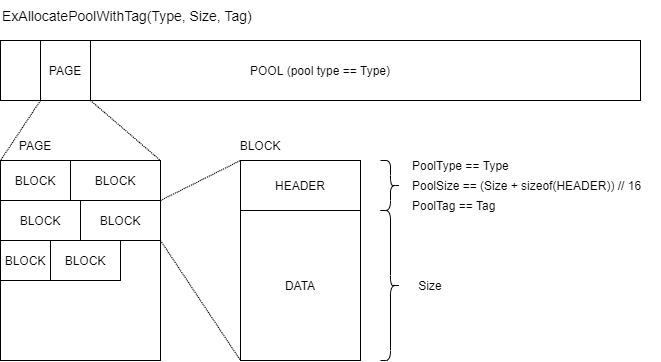
\includegraphics[scale=0.7]{images/pooltag.png}
\end{figure}

The pool that is relevant to the kernel data is called the non-paged pool. This
pool's pages are never paged out to disk and contain many kernel objects.  The
header of blocks allocated inside this pool will have the type value equal to
2. Kernel objects are allocated inside this pool with a tag hard-coded inside
the Windows source-code. Their tags and the structure are described in the
Table \ref{tab:pooltag}.

\begin{lstlisting}[language=windbg,caption=\texttt{\_POOL\_HEADER} in Windows 64-bit,float,floatplacement=H]
kd> dt _POOL_HEADER
nt!_POOL_HEADER
   +0x000 PreviousSize     : Pos 0, 8 Bits
   +0x000 PoolIndex        : Pos 8, 8 Bits
   +0x000 BlockSize        : Pos 16, 8 Bits
   +0x000 PoolType         : Pos 24, 8 Bits
   +0x004 PoolTag          : Uint4B
\end{lstlisting}

\subsection[Global list]{Global list}

Windows has several global lists to control the systems, the head (pointer) of
these lists is saved inside global variables in the kernel. For processes,
Windows has two circular doubly linked lists, indexed by
\texttt{PsActiveProcessHead}, \texttt{KiProcessListHead}.  There is also a
handle table list, \texttt{HandleTableListHead}, where each handle has a
pointer to \texttt{\_EPROCESS}. Kernel modules are also stored inside the
\texttt{PsLoadedModuleList}.

\subsection[Debug symbols]{Debug symbols}

The Windows source code is not publicly available, however Windows distributes
debug symbols for researching purposes. These debug symbols contains the offset
to global variables, functions and structures layout. The symbols are compressed
into a file called program database, or \textit{PDB}, with the extension
\texttt{.pdb}. The instruction to extract the file is limited described
\cite{microsoft-pdb}, but public works have been done and parsers are
available.

A PDB file is unique to one specific version of a kernel module. The PDB file
for the main kernel module is named \texttt{ntkrnlmp.pdb} for the kernel module
\texttt{C:\textbackslash \textbackslash Windows \textbackslash System32
\textbackslash ntoskrnl.exe}. The binary \texttt{ntoskrnl.exe} is different
across Windows updates. Downloading a specific PDB file for the kernel requires
the module's id, \textit{GUID}, and \textit{age}. GUID and age are parsed from
the binary in the RSDS section of a PE file \footnote{Executable file in
Windows OS}. In the same Windows version, specifically the Windows minor
version, structures layout are the same, but addresses to global variables and
functions are different.  Across different Windows' major version, huge changes
in structure layout, new functions and variables were introduced, and old ones
were removed. This is why downloading the correct PDB file for the current
machine is better than hardcoding the addresses, and members offset.

The Microsoft PDB server hosting the PDB files is located at
\url{https://msdl.microsoft.com/download/symbols}. To download the main kernel
module, we need to build the request URL as defined in Listing
\ref{lst:downloadpdb}. After that, parsing the PDB can be done using public
libraries, PDB parser by Brendan\cite{pdbparse} or PDB by Will
Glynn\cite{pdbrust}.

\begin{lstlisting}[language=cpp,caption=Download PDB file,label={lst:downloadpdb},float,floatplacement=H]
const string root_url = "https://msdl.microsoft.com/download/symbols/";
const string pdb_name = "ntkrnlmp.pdb";
const string guid = "XXXX";
const string age = "01";

const string download_url = root_url + pdb_name + "/"
                          + guid + age + "/"
                          + pdb_name;
\end{lstlisting}

\section[Prevention]{Prevention}

To prevent malware infiltration, both the Windows development team and
Anti-Virus vendors have tried to apply new technology to secure the operating
system. Here we list some advancement that has helped minimize the spread of
malware.

\subsection[Signature enforcement]{Signature enforcement}

In the past, drivers can be loaded on the system with only an admin privilege.
It was a bad practice, any driver, trusted or untrusted, can be loaded inside
Windows. Windows then forces driver creators/distributors to sign their drivers
using a Windows certificate to prevent untrusted drivers. Signing the driver
costs money and includes a code review that would prevent a malicious driver
created.

However, some malware writers are brilliant, they could reuse a legitimate
driver with vulnerability and \textit{exploit} the driver to make it work as
they wanted. The driver is trusted, but the bug inside the driver is used as an
attack vector. An example is RobinHood (2020) malware reused the
\texttt{GDRV.SYS} driver from Gigabyte \cite{robinhood}.

\subsection[Patchguard]{Patchguard}

Windows prevents malware from modifying kernel components with Patchguard.  In
the past, malware used to \textit{patch}, modify, some kernel components to
gain control of the system.  It was prevented after Windows introduced
Patchguard, a way to detect edits in the kernel code and crash the system when
editing detected.

Although this was a good approach, Windows still has some failure. The report
on malware bypassing Patchguard is GhostHook (2017) \cite{ghosthook}, and two
research to bypass the Patchguard are InfinityHook (2019) \cite{infinityhook},
and ByePg (2019) \cite{byepg}.

\subsection[On-access scanning]{On-access scanning}

On-access scanning is a technique developed by Anti-Virus vendors to scan the
file for malware evidence on accessing the file. They installed a hook in the
Windows API for file access, and scan the file on any read/write access. If the
file matches a previously defined signature, the Anti-Virus will prevent access
and warn the user for removal. The algorithm is illustrated in Figure
\ref{fig:onaccessscan}, this algorithm is used by McAfee Anti-Virus
\cite{onaccessscan}.

\begin{figure}[h]
  \centering
  \caption{McAffee On-access scanning}
  \label{fig:onaccessscan}
  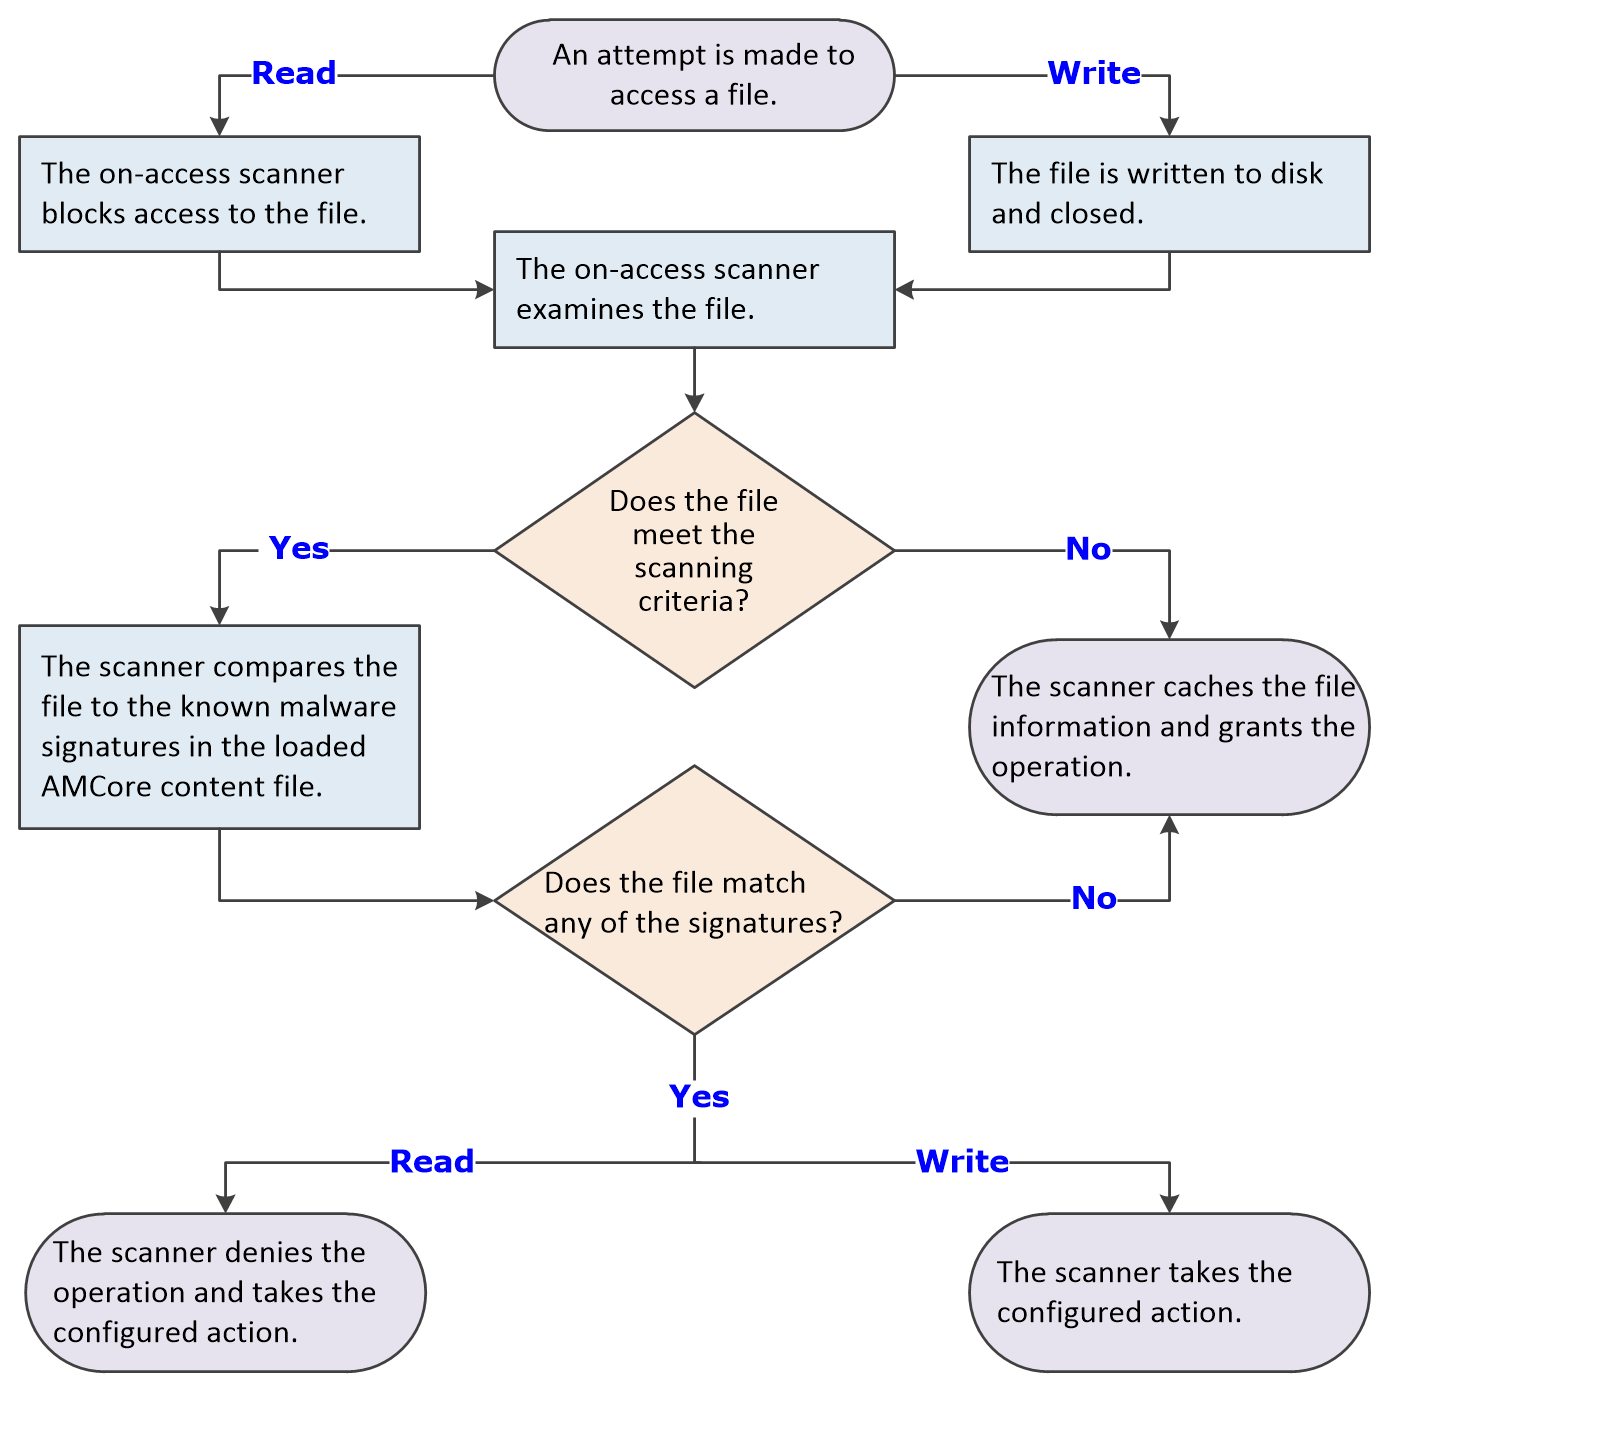
\includegraphics[scale=0.8]{images/onaccessscan.png}
\end{figure}

Because the scan depends on the pre-defined signature, a new malware could
bypass these rules if it uses a novel method to infect or hide. The rules can
be bypassed by applying obfuscation in the malware code, which hides traces of
evident behavior.

Scanning for signature using machine learning is still a new method, and even
though some vendors tried, the progress is not much positive. A security
researcher has created a sample malware bypassing the Cylance Smart Anti-Virus
in less than 15 minutes \cite{cylance}.


\chapter[Hidden malware and memory forensics]{Hidden malware and memory forensics}

Malware has many ways to run inside the system. It can create a process, create
a thread, load a library, or run a driver. A hidden malware will make these
objects can not be found when using Windows API or by traversing the legacy
lists.  For example, there are Windows APIs that can get information on
processes, threads, libraries, drivers, \texttt{EnumProcesses},
\texttt{Thread32First}, \texttt{EnumDeviceDrivers},
\texttt{NtQuerySystemInformation}. Malware will try to remove itself from these
API results. Thus, if an inspection system uses these API, the malware present
is not shown. To reveal the malware, one has to use forensics methods,
including but not limited to memory forensics.  In this chapter, we present in
technical terms how malware interfere with the system in order to hide and how
forensics investigators can find them using memory forensics.

\section[Process hiding]{Process hiding and rootkits}

In this section, we review the techniques used by malware to hide themselves
both on user space and kernel space. Most malware tries to infiltrate the
kernel space because it gives them more power to the system. These types of
malware running in kernel space are often referred to as rootkits. Rootkits are
hard to detect because they often hide from global lists.

\subsection[SSDT hooking]{SSDT hooking}

SSDT, short for System Service Descriptor Table, is a system call table in
Windows. SSDT hooking is the way malware rewrite the table and edit some
entries to the malware's function. A better way of rewriting is editing the
function into jumping or calling the malware's function. Of course, the malware
function must somehow perform the system function so that the OS can still be
running. In Figure \ref{fig:ssdt}, we show how SSDT hooking is done. The figure
shows a function in the SSDT is hooked and pointed to a function inside
\texttt{malicious.dll}.

\begin{figure}[h]
  \centering
  \caption{SSDT hooking}
  \label{fig:ssdt}
  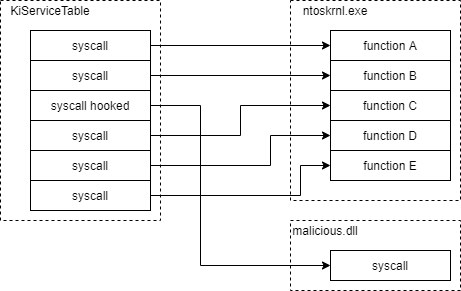
\includegraphics[scale=1]{images/ssdt.png}
\end{figure}

On p32-bit systems, each thread has a different SSDT, which can be edited (by
kernel process). Because this table is only visible to one thread, the malware
can modify it without changing the system table.

SSDT hooking is stealth and dangerous. A hooked SSDT function can alter the
result returned to hide the malware. As bad as it could be, many years ago
Anti-Virus software used this to monitor system calls
\cite{case2020hooktracer}. They track the calls to SSDT, e.g., the create file
system call and monitor what file is being created and apply some checks to see
if the action will harm the system, e.g., writes a malware to file.

\subsection[IRP hooking]{IRP hooking}

Each kernel driver has a list of 28 major functions used for communicating with
other processes, editing any of the 28 major functions is called IRP hooking.
IRP, \textit{I/O Request Packets}, is the data sent when the user application
communicates with the driver. IRP contains the index to the 28 major functions
to ask the driver to perform. A malware could change the major function list so
that the driver calls the malware's function.  IRP hooking is done either by
replacing the pointer or editing the function into jumping or calling the
malware's function. An advanced technique of IRP hooking, the malware allocates
a small section inside the driver and writes the malware's code then rewrites
the IRP functions into this code. Figure \ref{fig:irp} shows how IRP hooking is
done.

\begin{figure}[h]
  \centering
  \caption{IRP hooking}
  \label{fig:irp}
  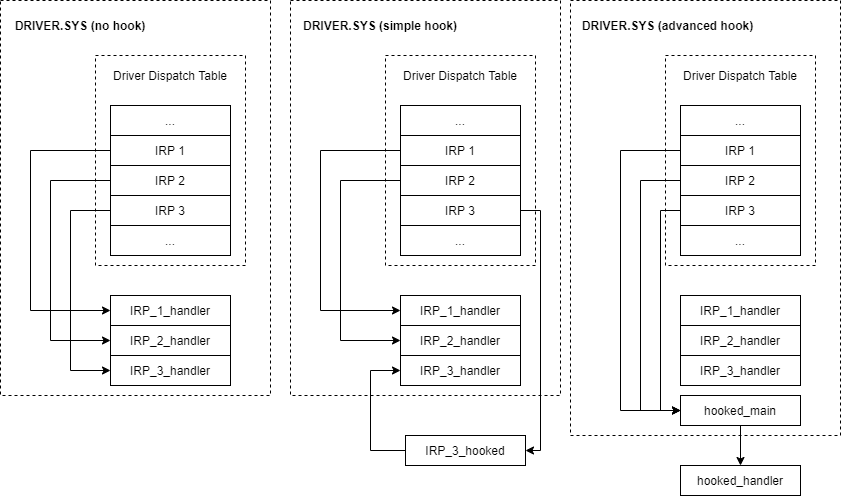
\includegraphics[scale=0.5]{images/irp.png}
\end{figure}

\subsection[DKOM]{DKOM}

DKOM is short for Direct Kernel Object Manipulation. It is when a malware
rewrites the kernel object members. One of the most used tricks related to DKOM
is removing object(s) from the linked list of the object, as shown in Figure
\ref{fig:dkom}.

\begin{figure}[h]
  \centering
  \caption{DKOM remove a node from linked list}
  \label{fig:dkom}
  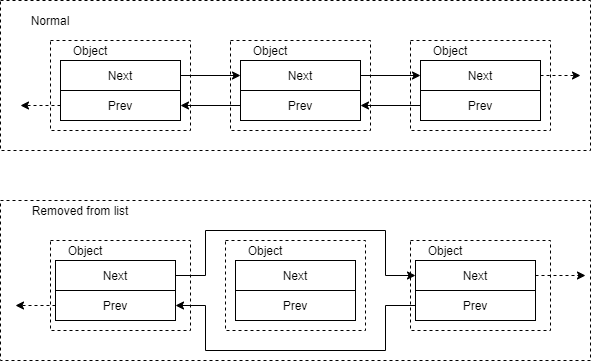
\includegraphics[scale=0.7]{images/dkom.png}
\end{figure}

The process list is a doubly-linked list, by removing the index to the desired
process malware can hide from windows API enumeration and list traversing.

The doubly-linked lists of loaded modules, namely \texttt{in load}, \texttt{in
memory}, \texttt{in initilization}, can all be edited to remove the module. A
naive malware will remove itself from the \texttt{in load} list, but a
comparison with the other two lists can reveal the hidden module. A better
hiding malware will try to remove itself from these three lists.

If the malware wants to hide one of its threads, it can remove the thread from
the threads list, the pointer to the thread list is \texttt{ThreadListHead} in
\texttt{\_EPROCESS}.

Removing a node from the linked list is a common task, but DKOM is not limited
to these techniques, the malware can edit many members. An old
research\cite{robussignature} made by Brendan on Windows XP reveals that of the
72 selective members from selective structures, 29 members can be modified
without affecting, crashing, the system.  However, this research needs to be
updated with Windows 10. From the research results, malware can edit many
members, some of which could hide from the system without breaking the system.

\section[Memory Forensics]{Memory Forensics}

With all the preventions, malware still finds a way to bypass the security
setup and infect the system. When such an event occurs, a skilled technician
will begin analyzing the system. To start the investigation, they would need to
take the physical memory content of the system and analyze the content looking
for prominent malware. This is called memory forensics, a sophisticated process
done by a team of security researchers when a breach occurs or when an unknown
factor compromises the system.

\subsection[Memory acquisition]{Memory acquisition}

The first step in memory forensics is capturing the content of physical memory.
This step is often called as \textit{memory acquisition}. The goal was to load
the RAM data inside a file. There are multiple ways \cite{memoryAcquisition} to
do this in a running machine using a kernel driver:

\begin{enumerate}
\item Read \texttt{\textbackslash\textbackslash.\textbackslash PhysicalMemory}
\item Use \texttt{MmMapMemoryDumpMdl}
\item Use \texttt{MmMapIoSpace}
\item PTE remapping
\end{enumerate}

The RAM is a device, and Windows exposes the device as a file with the absolute
path \texttt{\textbackslash\textbackslash.\textbackslash PhysicalMemory}. By
reading this file, we are accessing the RAM itself. However, Windows prevented
reading this file. The second and third method maps physical page(s) to the
kernel space, the content is sent back to the user space to write out the file.
The fourth method is a technique described by Michael Cohen and Johannes
Stüttgen \cite{pteremap} to capture the memory using the PTE, page table entry.

Most memory acquisition tools are closed source, the one open-source memory
acquisition tool is WinPmem \cite{winpmem} and using the third and fourth
method to capture the RAM. WinPmem's author also encourages using the PTE
remapping method for better results. Other programs often used for memory
acquisition are \texttt{DumpIt} by Moonsol, \texttt{FTK Imager} by AccessData,
\texttt{Belkasoft RAM Capturer} by Belkasoft.

Hypervisor, VirtualBox or VMWare, can generate the memory file.  Although the
memory file format is different from each virtual machine implementation, the
documentation of the file format is available online.

The last way to acquire the memory content is through Windows debug mechanism.
Windows has an option to generate the memory file when the system crash, if
this option is on, Windows will produce the file at \texttt{C:\textbackslash
Windows\textbackslash MEMORY.DMP} on system crash. Windows also has multiple
option to the memory file, such as the \textit{full dump}, \textit{mini dump},
\textit{kernel dump}. These files are not officially documented by Windows and
intended to be used by Windows debugger, but researchers have reversed the file
format for forensics purposes \cite{mdmpfile} \cite{dmpfile}.

\subsection[KDBG]{KDBG}

KDBG is a Windows structure for debugging purposes, this structure contains
pointers to many kernel essential components, such as the list of processes.
Finding this structure in the memory file will give some insight into the
system.  This structure can be found using the four-byte ``KDBG'' in Windows
versions before 8. In Windows 8 and above, the structure is encoded and makes
it more challenging to find the structure. However, by brute-scanning and
brute-decoding \cite{kdbgEncoded}, one can still find the structure.

\subsection[Pool tag scanning]{Pool tag scanning}

As described in Section \ref{sec:pool}, each block has a pool header contains a
four-byte tag. By scanning for a specific tag value that the OS uses to
allocate for a kernel structure, we can search for all the object allocated,
and sometimes de-allocated but not overwritten. Each tag-block matches should
be further checked for validity, the pool body size (block size subtract the
pool header size) should be bigger than the object holding (if the object is an
executive object), or equal to the object.  Optional checks for pool type value
are done with objects usually allocated in one pool section.  E.g.,
\texttt{\_EPROCESS} is always allocated inside the non-paged pool section,
hence the pool type is 2. This technique is called \textit{Pool tag scanning}
\cite{pooltagscan}, and often done by a full search in the memory file. In
2016, Sylve, Joe T and Marziale, Vico and Richard III, Golden G
\cite{sylve2016pool} improved this technique by locating the range of the
non-paged pool region and scan only the pages that are valid. They named the
technique \textit{Pool tag quick scanning}.

The pool tag quick scanning research is conducted on Windows Vista and 8, we
extended the findings of these ranges on Windows XP, 7, 8, and 10 (all versions
from 2015 to 2020), with reference from the Rekall project. The result can be
found in Table \ref{tab:nonpaged}.

\begin{table}[]
\begin{tabular}{lll}
\hline
Windows version & Pool start                      & Pool end                      \\ \hline
XP              & \texttt{nt!MmNonPagedPoolStart} & \texttt{nt!MmNonPagedPoolEnd} \\
7, 8, 8.1       & \texttt{nt!MiNonPagedPoolStart} & \texttt{nt!MiNonPagedPoolEnd} \\
10 2015         & \texttt{nt!MiState}
                & \texttt{nt!MiState} \\
                & \texttt{->SystemNodeInformation}
                & \texttt{->SystemNodeInformation} \\
                & \texttt{.NonPagedPoolFirstVa}
                & \texttt{.NonPagedPoolLastVa} \\
10 2016-2019    & \texttt{nt!MiState}
                & \texttt{nt!MiState} \\
                & \texttt{->Hardware}
                & \texttt{->Hardware} \\
                & \texttt{.SystemNodeInformation}
                & \texttt{.SystemNodeInformation} \\
                & \texttt{.NonPagedPoolFirstVa}
                & \texttt{.NonPagedPoolLastVa} \\
10 2020         & \texttt{nt!MiState}
                & \texttt{nt!MiState} \\
                & \texttt{->Hardware}
                & \texttt{->Hardware} \\
                & \texttt{.SystemNodeNonPagedPool}
                & \texttt{.SystemNodeNonPagedPool} \\
                & \texttt{.NonPagedPoolFirstVa}
                & \texttt{.NonPagedPoolLastVa} \\ \hline
\end{tabular}
  {\raggedright \texttt{nt!foo} is the address of \texttt{foo} in kernel space
    \par}
  {\raggedright \texttt{nt!MiState} is a pointer to the type
  \texttt{\_MI\_SYSTEM\_INFORMATION}, this structure layout is different with
  each Windows 10 releases \par}
  {\raggedright \texttt{nt!MiNonPagedPoolStart} or
  \texttt{nt!MiNonPagedPoolStartAligned} both valid for Windows 7, 8, 8.1. Aligned
  version points to the first valid page in the pool \par}

  \caption{Non paged pool start and end}
  \label{tab:nonpaged}
\end{table}

Pool tag scanning is often used to ensure there is no process hiding from the
kernel list by simple removal. Comparing the pool tag scanning result with the
list traversing, we may be able to reveal unlinked objects from the global
list. However, pool tag scanning can be used to reveal other objects often not
reside on any list. These can be internet-related structures, kernel callbacks.
Although Windows does not document this structure, many people have studied the
Windows source code (by reversing) and came up with structure definitions and
reasonable names. In Table \ref{tab:pooltag}, we list the tags and the
structure where pool tag scanning is often used to find. These tags are used in
the Volatility framework.

\begin{table}[]
\begin{tabular}{llll}
\hline
  Structure                 & Structure Name                     & Pool Tag (new) & Pool Tag (old)        \\ \hline
  Driver Object             & \texttt{\_DRIVER\_OBJECT}          & Driv           & Dri\textbackslash xf6 \\
  File Object               & \texttt{\_FILE\_OBJECT}            & File           & Fil\textbackslash xe5 \\
  Process                   & \texttt{\_EPROCESS}                & Proc           & Pro\textbackslash xe3 \\
  Thread                    & \texttt{\_ETHREAD}                 & Thre           & Thr\textbackslash xe5 \\
  Modules                   & \texttt{\_LDR\_DATA\_TABLE\_ENTRY} & MmLd           &                       \\
  TCP endpoint              & *\texttt{\_TCP\_ENDPOINT}          & TcpE           &                       \\
  TCP listener              & *\texttt{\_TCP\_LISTENER}          & TcpL           &                       \\
  UDP endpoint              & *\texttt{\_UDP\_ENDPOINT}          & UdpA           &                       \\
  TCP connection            & *\texttt{\_TCPT\_OBJECT}           & TCPT           &                       \\
  Notification Packet       & *\texttt{\_NOTIFICATION\_PACKET}   & IoFs           &                       \\
  Shutdown Packet           & *\texttt{\_SHUTDOWN\_PACKET}       & IoSh           &                       \\
  Generic callback          & *\texttt{\_GENERIC\_CALLBACK}      & Cbrb           &                       \\
  DbgPrint callback         & *\texttt{\_DBGPRINT\_CALLBACK}     & DbCb           &                       \\
  Registry callback         & *\texttt{\_REGISTRY\_CALLBACK}     & CMcb           &                       \\
  Hardware profile callback & *\texttt{\_NOTIFY\_ENTRY\_HEADER}  & Pnp9           &                       \\
  Device interface callback & *\texttt{\_NOTIFY\_ENTRY\_HEADER}  & PnpD           &                       \\
  Target device callback    & *\texttt{\_NOTIFY\_ENTRY\_HEADER}  & PnpC           &                       \\
\hline
\end{tabular}
  {\raggedright *: This structure is not documented by Windows, the name is taken
  from Volatility framework \par}
  \caption{Comprehensive list of pool tag and corespondent structure}
  \label{tab:pooltag}
\end{table}

\subsection[SSDT and IRP hook detection]{SSDT and IRP hook detection}

SSDT hooking is dangerous in a way it can modify the kernel system call
behavior.  Detection of SSDT involves finding the system table and locate the
function address between loaded modules.The SSDT is located at
\texttt{KiServiceTable}, with \texttt{KiServiceLimit} elements of 32-bit value.
Every element is an offset to the function of the SSDT. To retrieve the address
of the function, we follow Listing \ref{lst:ssdt}.


\begin{lstlisting}[language=cpp,caption={Retrieve SSDT functions},label={lst:ssdt},float,floatplacement=H]
int32_t* KiServiceTable;
int KiServiceLimit;
void* ssdt[KiServiceLimit];
for (int i = 0; i < KiServiceLimit; i++) {
  ssdt[i] = (void*) ((int64_t)KiServiceTable + (KiServiceTable[i] >> 4));
}
\end{lstlisting}

After recovering all the functions in the system call table, we will check
every loaded module of type \texttt{\_KLDR\_DATA\_TABLE\_ENTRY} and see if the
address of the function is in the range of the \texttt{DllBase} and
\texttt{DllBase + Size}, if the address is between this range, the function is
in this module.  Because these are system calls, the functions should reside in
the kernel module, \texttt{ntoskrnl.exe}. If some functions reside in another
module, the SSDT probably hooked. Some malware even modify the function
instruction to jump or call to itself, this can be check by dumping several
bytes at the function address and decompile into machine code checking for jump
instruction and check the referenced address module.

IRP hooking is in driver 28 major functions. To detect this type of hook, we
list the 28 major functions searching for the loaded modules containing these
functions. It should be noted that the driver should either have the IRP
functions belongs to the driver or the kernel modules. If the functions are of
another module, then it was probably hooked. If the malware patch the
underlying function to jump or call itself, decompile the first few bytes
looking for such instruction and check the referenced address' module. For
the advanced IRP hooking method, this can only be detected after reversing the
function being hooked.

% To make the result easier to read and understand, the loaded module are parsed
% to get the exported symbols. When printing out the result, the module name with
% the function name will be printed out.

\subsection[Unloaded kernel drivers]{Unloaded kernel drivers}

There are some cases where malware load and unload the kernel driver almost
immediately (Rustock). In these scenarios, looking inside the unloaded driver
list might shed some light on this type of malware. Windows stores a list of
unloaded kernel drivers, the pointer to the list is located at
\texttt{MmUnloadedDrivers}. The list contains at most 50 members sized 0x28
bytes, the first 0x18 bytes in each member is of type
\texttt{\_UNLOADED\_DRIVER}.  \texttt{\_UNLOADED\_DRIVER} only contains the
name of the driver and the start and end address of the driver, the
\texttt{\_DRIVER\_OBJECT}, in most cases, is deallocated. If lucky, pool tag
scanning may show drivers unloaded, but it is usually not the case.


\chapter[Related Works]{Related works}
\section[Volatility]{Volatility}

Volatility \cite{volatility} is an open-source forensics tool first developed
by Aaron. The four developers of this project also publish the book on memory
forensics, The Art of Memory Forensics.

Volatility is written in Python 2, and the project is being rewritten (2020) in
Python 3. The project is a result of many research in memory forensics in
Windows, Linux, and MacOS. Volatility only works on memory file, and support
many memory file formats.

To find malware in Windows, Volatility has commands to list processes, kernel
modules, inspect the SSDT and IRP, and list unloaded drivers. Volatility also
employs pool tag scanning to find processes, threads, drivers, kernel modules,
network connections, kernel callbacks. Volatility has a command to compare the
process lists produced by traversing different process list and pool tag
scanning for processes, \texttt{psxview}.  Figure \ref{fig:volatility} shows
the sample output of the Volatility's \texttt{psxview} commands.

\begin{figure}[h]
  \centering
  \caption{Volatility}
  \label{fig:volatility}
  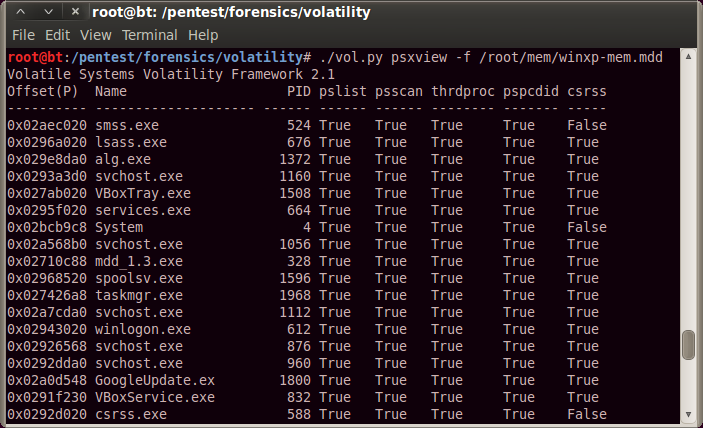
\includegraphics[scale=0.5]{images/volatility.png}
\end{figure}

Volatility is a versatile and powerful tool ever created to tackle the memory
forensics. It can work on memory dumps of different Windows versions and help
investigators explore many data related to the system.

\section[Rekall]{Rekall}

Rekall open-source project by Google \cite{rekall} is the second choice in
memory forensics.  Rekall is also written in Python 2 and provides almost the
same functionalities that Volatility has. Rekall uses the debug symbols to
resolve the structures layout and global variable offsets in Windows analysis.
One withdrawal from Rekall is probably the installation, where Rekall is harder
to install and use than Volatility.

Rekall has a memory capture module called WinPmem, which is also a kernel
driver for doing live forensics. On doing live memory forensics, WinPmem
creates a device at \texttt{\textbackslash\textbackslash .\textbackslash pmem}
and Rekall will perform the forensics on the device.

Rekall performs live forensics by mapping every physical memory pages and binds
the read operation to \texttt{\textbackslash\textbackslash .\textbackslash
pmem} in \texttt{IRP\_MJ\_READ}. When the user application read the file at an
offset, WinPmem driver will map the required physical page and copy to the
output buffer.

\section[Memtriage]{Memtriage}

Memtriage \cite{memtriage} is a wrapper around the Rekall WinPmem driver and
Volatility to do live forensics with Volatility.  This project can make
Volatility works on live systems with limitations. There have been crashes
reported on some Windows versions.


\section[SysInternal]{SysInternal}

Sysinternals \cite{sysinternal} is a suite of programs made by Mark
Russinovich, now redistributed by Windows. Two programs that are used by
malware analysts to inspect the system are Process Explorer and Process
Monitor.  Process Explorer is a Task manager with verbose information. Process
Explorer uses Windows API to query the systems for process and threads
information.  Process Monitor captures events by Windows and displays them in a
GUI. Process Monitor can capture process/thread creation, termination, file
access, registry access, network activities and many more. On a live machine,
Process Monitor is handy to know what process is doing so that malware analysts
can narrow down process by process to find the malware writing registry values,
edit a file, or connecting to a remote server.


\begin{figure}[h]
  \centering
  \caption{Process Explorer}
  \label{fig:processexp}
  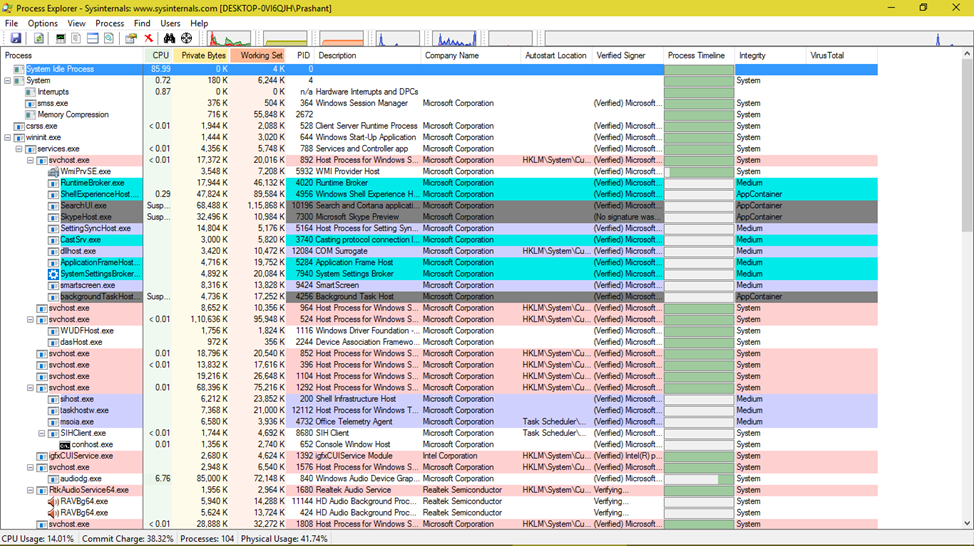
\includegraphics[scale=0.4]{images/processexp.png}
\end{figure}

\begin{figure}[h]
  \centering
  \caption{Process Monitor}
  \label{fig:processmon}
  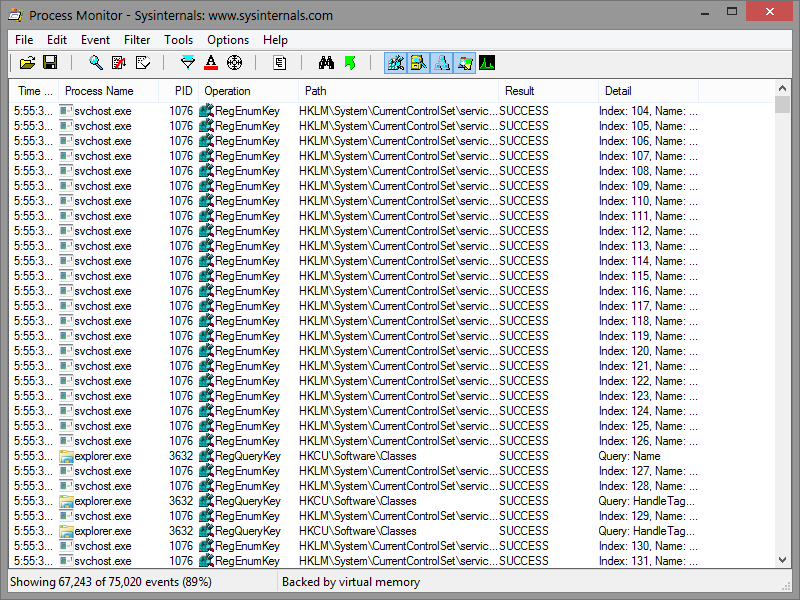
\includegraphics[scale=0.5]{images/processmon.png}
\end{figure}

\section[Process hacker]{Process hacker}

The Process Hacker \cite{processhacker} is an open-source project maintained by
Wen Jia Liu and Steven G. The goal of this project is to give the user a tool
to monitor system resources, debug software, and detect malware. Process Hacker
has a graphical user interface to inspect processes, network connections, file
access. Process Hacker also uses a kernel driver to capture stack traces,
enumerating process handler more efficiently, retrieving names for file
handlers and EtwRegistration objects, and setting handle attributes.

Process hacker does not use any forensics methods to detect malware, but either
using more verbose information into the system to let the user know what
processes are doing.


\begin{figure}[h]
  \centering
  \caption{Process Hacker}
  \label{fig:processhacker}
  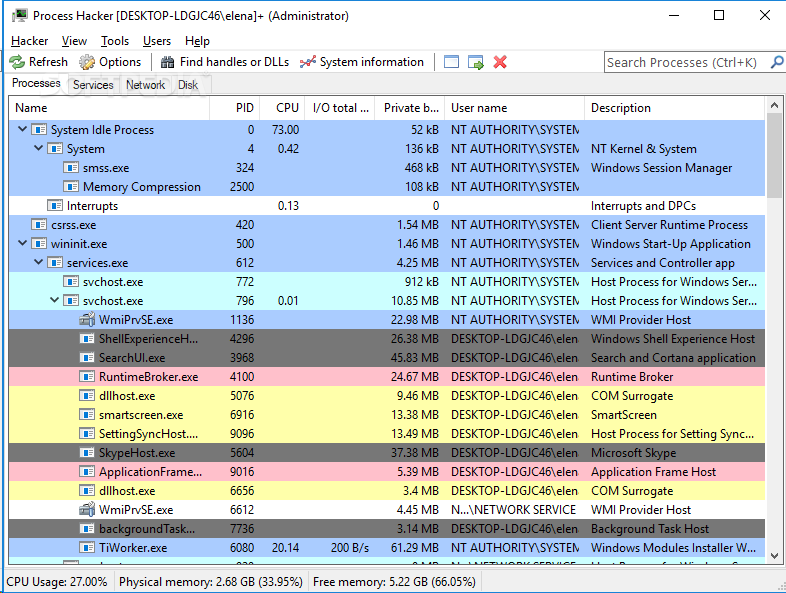
\includegraphics[scale=0.7]{images/processhacker.png}
\end{figure}



\chapter[Tools and technology used]{Tools and technology used}

This thesis's outcome can not be achived without the tools and technologies
used to develop, debug and test. With the right tools, we can make the work
easier and faster. In this chapter we list the tools and technologies used to
make our desire forensics tool.

\section[The C++ language]{The C++ language}

C++ is an old language, first developed by Bjarne Stroustrup in 1985 as a
complement to the C language. C++ delivers better type checking and more
\textit{notational support}. With its strong compatibility with C and its
strictness, C++ is a better programming language for enterprise-level projects.

The transition from C to C++ is slowly adapted to OS programming. The Windows
operating system supports writing drivers using C++. However, using C++ in the
kernel is very difficult. In the kernel space, there is no runtime. In other
words, no standard library, no exception handling, no constructor for global
objects.  Although most C++ features are still available: classes, range-for
loop, lambda, templating.

Writing the kernel driver in C++ will make the code easier to manage and
extend. That is why we are using C++ when developing the kernel driver.

\section[The Rust language]{The Rust language}

Rust is a new language developed by Graydon Hoare. It first appears in 2010.
The language is designed to eliminate the bad design in concurrent programming
languages while retaining the program's efficiency and speed.  Regardless of
its age, many successful projects have been made with Rust. Rust makes the code
safety from compile-time to runtime by checking for memory access during
compilation. Rust captures attention from system programmer, from Microsoft to
Linux developers, all are considering using Rust in their future projects and
planning to use Rust with the system.

We use Rust to develop the user application. Rust can interface C structures
and call native Windows API easily. With the speed comparable to C++ and the
safety that Rust gives, choosing Rust was a brilliant idea.

\section[WinDbg]{WinDbg}

WinDbg is a debugger, a tool used to debug other programs, made by Microsoft.
WinDbg was first developed for the developer to inspect the crash dump produced
when the Windows crash. However, it can later be used to debug a running
machine through a wire connection. WinDbg fetches the debug symbols
automatically and use it to help developers debug the problem. In 2017,
Microsoft announced a remake of WinDbg, WinDbg Preview, with stunning graphics
and new features.

\section[VirtualBox]{VirtualBox}

We are developing a tool used inside the kernel space. It is advised to use an
isolated environment for testing. By using a hypervisor, a software that
simulates the hardware to run an OS, we get an isolated environment.
VirtualBox is a hypervisor distributed under Oracle and is free to use.
VirtualBox can run a wide range of Windows versions, which is suitable for
testing multiple Windows versions. VirtualBox can be set up to debug the
running operating system with WinDbg, as in Figure \ref{fig:windbg}.

\begin{figure}[h]
  \centering
  \caption{WinDbg debugging Windows 7 on VirtualBox}
  \label{fig:windbg}
  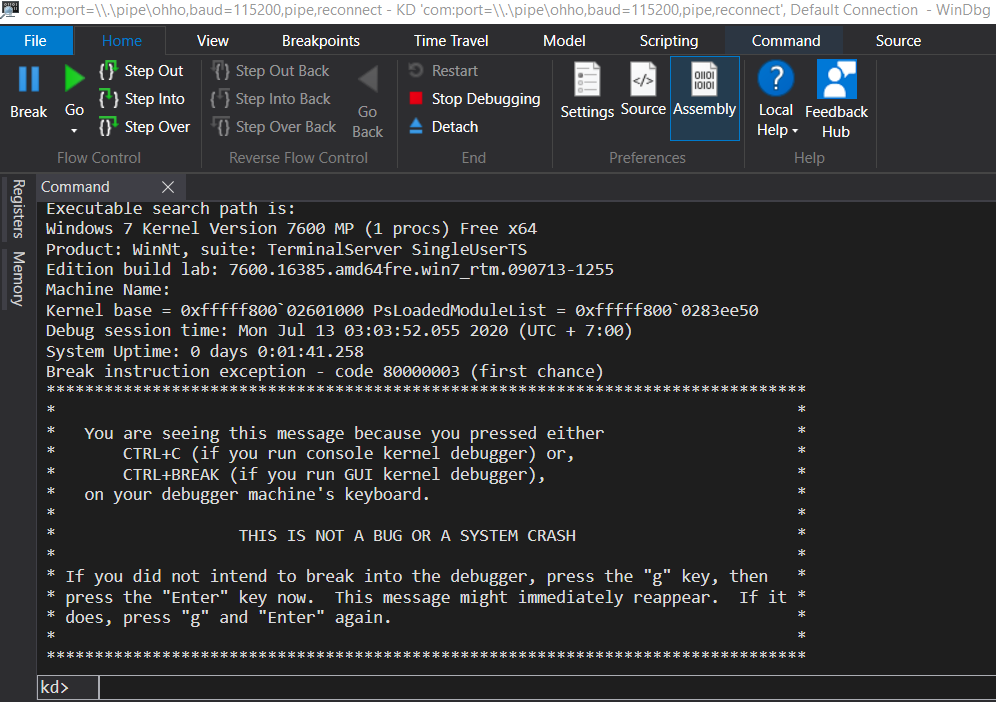
\includegraphics[scale=0.4]{images/windbg.png}
\end{figure}

\chapter[Solution]{Solution}

Rekall on Chapter 4, the current tools used for finding hidden process are
forensics tools and live system queries. Forensics tools requires the memory
file to be extracted and the live system queries misses information that could
only be found when doing forensics. We hope to deliver a quick and nice
solution to perform memory forensics on a live machine.

This chapter introduces LPUS, a system capable of doing live memory forensics
without extracting the RAM contents. In short, LPUS uses a kernel-mode driver
to locate the kernel base and efficiently walks the kernel structures without
breaking the systems. Since LPUS can locate the appropriate kernel address to
be accessed, it does not require the memory file. LPUS uses forensics to help
users find malware by implementing some standard scans and collecting
information crucial for identifying hidden malware.

\section[Prerequisites]{Prerequisites}

LPUS has some prerequisites for the environment running on. Before moving on to
the LPUS system, we will briefly go through each prerequisite and explain why.

\subsection[Operating system]{Operating system}

Windows machine running LPUS must be 7 or above. While the Windows server is
not tested, the Windows home machine with version 7 or above is guaranteed to
execute LPUS without any problem.  The reason why LPUS does not support Windows
XP and the lower Windows version is that the third parties that LPUS depends
on. Third-parties used by LPUS deprecate the old Windows version by using newer
Windows API. Although we can rewrite the module to use the old Windows API
which will work on more Windows version, the work burden would be too much.

\subsection[Requirements for the driver]{Requirements for the driver}

The LPUS kernel-mode driver must be signed or \textit{test mode} is on.  In
Section 2.3.1, we discussed how Windows enforces driver signing to protect
untrusted drivers from loading into the system. Thus, the LPUS kernel driver
must be signed if we want to load in the system. In this thesis, we want to
demonstrate LPUS's usability, which is why signing the driver is not needed,
and instead, we use a development environment for testing the driver. This test
environment is called test mode, a feature which allows loading unsigned
driver. To enable the environment, one must enter \texttt{bcdedit /set
testsigning on} on an elevated command prompt and reboot the machine. On
rebooting, a small text read \texttt{Test Mode} will be visible in the bottom
right corner on the Desktop as in Figure \ref{fig:testmode}.

\begin{figure}[h]
  \centering
  \caption{Testmode enabled}
  \label{fig:testmode}
  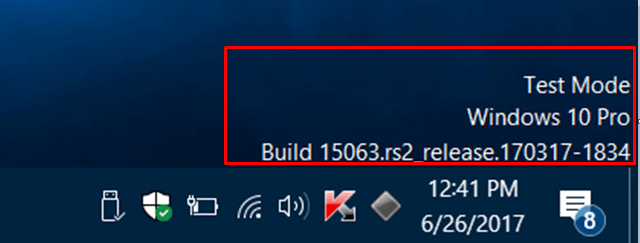
\includegraphics[scale=0.7]{images/testmode.png}
\end{figure}

\subsection[Run LPUS as Administrator]{Run LPUS as Administrator}

LPUS must be run as Administrator because LPUS edits the registry and uses a
special privilege to load the driver. Editing the registry can only be done if
the application is running as an Administrator. If the registry is already set,
LPUS can be run by a user having a special privilege, \texttt{SeLoadDriver}.
However, for convenience, LPUS should be run as an Administrator.

\section[LPUS system]{LPUS system}

In this section, we elaborate on the two LPUS components that the LPUS system
consists of, the kernel driver and the user application. We go through the
steps LPUS makes to enable live forensics and how LPUS can perform live
forensics without extracting the memory file. For convention, the kernel driver
will be called the \textbf{backend} and the user application will be called the
\textbf{frontend}. Here are the steps that LPUS takes from startup to
termination. (1) LPUS registers the registry keys and \textbf{loads the kernel
driver in the system}. (2) LPUS downloads and \textbf{loads the debug symbols}
on the current system.  (3) LPUS \textbf{finds the kernel base address}. (4)
LPUS uses the kernel base address to \textbf{perform forensics}. (5) LPUS
terminates. We will go through each step and analyze what LPUS does.

\subsection[Loading driver]{Loading driver}

LPUS loads the kernel driver on startup. Loading the kernel driver requires a
registry key containing the path to the driver and the load driver privilege
enabled. LPUS writes the registry key at
\texttt{HKEY\_LOCAL\_MACHINE\textbackslash System \textbackslash
CurrentControlSet \textbackslash Services \textbackslash lpus} with the
\texttt{ImagePath} value contains the path to the kernel driver as shown in
Figure \ref{fig:registry}. This registry key will be passed onto
\texttt{NtLoadDriver} as the first parameter to load the driver. To make the
driver loading success, LPUS will enable the \texttt{SeLoadDriver} privilege.
The \texttt{SeLoadDriver} is available if the user running LPUS is an
Administrator, however, the value is disabled. LPUS uses the code on Listing
\ref{lst:seloaddriver} to enable the privilege. After these operations, LPUS
has loaded the kernel driver onto the running system


\begin{figure}[h]
  \centering
  \caption{LPUS setup registry}
  \label{fig:registry}
  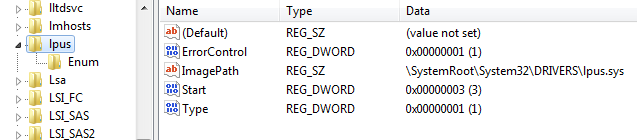
\includegraphics[scale=1]{images/registry.png}
\end{figure}

\begin{lstlisting}[language=rust,caption={Enable SeLoadDriver},label={lst:seloaddriver},float,floatplacement=H]
let str_se_load_driver_privilege = CString::new("SeLoadDriverPrivilege")
                                   .unwrap();
let mut token_handle: HANDLE = null_mut();
let mut luid = LUID::default();
OpenProcessToken(
    GetCurrentProcess(),
    TOKEN_ADJUST_PRIVILEGES,
    &mut token_handle,
);
LookupPrivilegeValueA(null_mut(),
                      str_se_load_driver_privilege.as_ptr(),
                      &mut luid);
let mut new_token_state = TOKEN_PRIVILEGES {
    PrivilegeCount: 1,
    Privileges: [LUID_AND_ATTRIBUTES {
        Luid: luid,
        Attributes: SE_PRIVILEGE_ENABLED,
    }],
};
AdjustTokenPrivileges(
    token_handle,
    0,
    &mut new_token_state,
    16,
    null_mut(),
    null_mut(),
);
CloseHandle(token_handle);
\end{lstlisting}

\subsection[Load debug symbols]{Load debug symbols}

After successfully loading the kernel driver, LPUS will download the debug
symbols for the system. LPUS parse the GUID and age for the kernel file
\texttt{C:\textbackslash \textbackslash Windows \textbackslash System32
\textbackslash ntoskrnl.exe} and builds the URL to download the PDB from the
Microsoft server as in Listing \ref{lst:downloadpdb}. After the file is
downloaded, LPUS uses a third-party PDB module to parse the downloaded PDB file
into a hashmap to index quickly. There are two hashmaps, the hashmap of global
variables and functions, and the hashmap of structure and members. The hashmap
of global variables and functions are indexed by the name of the symbol and
stores the offset to the symbol. For the hashmap of structures, the index key
is the structure name and stores the hashmap of members. The hashmap of a
member is indexed by the member name and stores the member's type and offset of
the member in the structure. Listing \ref{lst:pdbstore} shows the data
structure the debug symbols are stored.

\begin{lstlisting}[language=rust,caption={Stores debug symbols},label={lst:pdbstore},float,floatplacement=H]
// Symbol name -> Offset
type SymbolStore = HashMap<String, u64>;

// Struct name -> Hashmap(Member -> (Type, Offset))
type StructStore = HashMap<String, HashMap<String, (String, u64)>>;

struct PdbStore {
    pub symbols: SymbolStore,
    pub structs: StructStore,
}
\end{lstlisting}

\subsection[Setup communication and kernel base address]{Setup communication and kernel base address}

After loading the kernel driver and debug symbols, LPUS setups the connection
between the backend and frontend and search for the kernel base address. The
connection between the two is vital, and this is what makes LPUS capable of
querying the kernel space.

The backend and frontend communication is kernel-land and user-land
communication. The kernel-land cannot access the user-land and the user-land
cannot access the kernel land. To communicate with each other, they must have a
shared object, a physical file. Communicating using this physical file is the
same as socket programming between the server and a client. The packet is sent
by the user application in the form of an IRP. The driver receives the IRP and
the driver performs computation depends on the IRP action code.  Sending data
between the two also uses the IRP packet. The protocol must first be defined by
the user application to send or receive. There are four modes for transferring
data: \textit{in direct} for sending data to the driver, \textit{out direct}
for receiving data from the driver, neither for communication without data
transferring and bi-directional if the user application sends to and receives
from the driver.

To create the communication, the driver creates the physical file and user
application \textit{binds}, connect, to the file. Both frontend and backend
have to accept the set of action codes and data input-output to avoid crashing
the system. After that, the user application can call \texttt{DeviceIoControl}
to send the action code, the input buffer, the output buffer to the driver. The
code setting up the communication can be found on Listing \ref{lst:deviceio}.

\begin{lstlisting}[language=cpp,caption={Setup communication},label={lst:deviceio},float,floatplacement=H]
// Driver code
NTSTATUS
DriverControl(PDEVICE_OBJECT /* DriverObject */, PIRP Irp) {
  PIO_STACK_LOCATION irpSp = IoGetCurrentIrpStackLocation(Irp);
  ULONG controlCode = irpSp->Parameters.DeviceIoControl.IoControlCode;
  switch (controlCode) {
    // handle action
  }
}

NTSTATUS
DriverEntry(
    _In_ PDRIVER_OBJECT     DriverObject,
    _In_ PUNICODE_STRING    /* RegistryPath */
) {
  // ntUnicodeString   = "\\Device\\lpus"
  // ntWin32NameString = "\\DosDevices\\lpus"

  // creates the file device
  IoCreateDevice(
    DriverObject,             // Our Driver Object
    0,                        // We don't use a device extension
    &ntUnicodeString,         // Device name "\Device\lpus"
    FILE_DEVICE_UNKNOWN,      // Device type
    FILE_DEVICE_SECURE_OPEN,  // Device characteristics
    FALSE,                    // Not an exclusive device
    &deviceObject);           // Returned ptr to Device Object

  // make the file accessible from user space
  IoCreateSymbolicLink(&ntWin32NameString, &ntUnicodeString);

  // register function receiving IRP
  DriverObject->MajorFunction[IRP_MJ_DEVICE_CONTROL] = DriverControl;
}

// User application code
HANDLE f = CreateFile("\\\\.\\poolscanner", ...);
DeviceIoControl(f, controlCode, ...);
\end{lstlisting}

When the connection between the backend and frontend is established, the
frontend will send some required offset for the backend to get the kernel base
address.  To get the kernel base address, LPUS uses the process list. The
offset from the kernel base address to the process list head can be fetched
from debug symbols, with the address of the process list we can easily
calculate the kernel base address. This requires us to find the process list
head. The backend can get inside the process list by getting an
\texttt{\_EPROCESS} through calling \texttt{IoGetCurrentProcess}. From a node
inside the list, LPUS can search for the head by traversing through the list.
Unfortunately, this does not work so well, and the process list is a circular
linked list, there is no null at the end or at the front of the list, which
makes it challenging to find the head.  However, we have noticed an interesting
fact with \texttt{IoGetCurrentProcess}.  The process returned by calling
\texttt{IoGetCurrentProcess} is the process of interacting with the driver, and
the process loading the driver onto the system is the \texttt{System} process.
The \texttt{System} process, how convenient, is the first item in the process
list. By getting the \texttt{System} when the driver loads using
\texttt{IoGetCurrentProcess}, we only need to traverse back one time to get the
list head. When the list head address is found, a subtraction from the offset
parsed from the PDB file will result in the kernel base address. The backend
will now return the kernel base address to the frontend.

\subsection[Perform forensics]{Perform forensics}

Reaching this step, LPUS has successfully loaded the kernel driver in the
system space, prepared the debug symbols, set up the communication between the
backend and userland, and have the kernel base address. From now, LPUS can
perform forensics on the system.

With the kernel base address, LPUS can easily get and traverse every list,
inspect any global variable if the type of the variable is well-known. The list
of processes LPUS can access is \texttt{PsActiveProcessHead},
\texttt{KiProcessListHead}, and the \texttt{HandleTableListHead}. LPUS can
access the kernel list by reading \texttt{PsLoadedModuleList}. The SSDT table
can be accessed by reading \texttt{KiServiceTable}, as well as the unloaded
module list in \texttt{MmUnloadedDrivers}.

Pool tag scanning is feasible with LPUS. As shown in Table \ref{tab:nonpaged},
the start and end section of the non-paged pool are indexed by the kernel base
address. LPUS can easily fetch the range value and perform scanning in between
looking for four-byte value. Scanning in this region is safe, but we should
take precautions. The address in this region is virtual memory, some pages are
mapped in RAM, but some pages do not. Accessing the address where the page is
not in RAM will cause the system to crash with a violation \texttt{Page Fault
In Nonpaged Area}. LPUS tries to handle the situation by checking every page
aligned address before accessing the page. The page aligned address will be
checked using \texttt{MmIsAddressValid}. If the result is false, or the address
is invalid, this indicates the page starting at the address is not assigned a
physical page. LPUS skips a page on \texttt{MmIsAddressValid} returns false,
and other cases where the memory accessed passes the current page but the next
page is invalid.

Because LPUS possesses the kernel base address, LPUS can explore the kernel
space if it knows the exact address of kernel variables and follows the
pointers inside kernel structures. With this forensics possibility, we show
more on what LPUS can do in Chapter 7.

\subsection[Termination]{Termination}

After forensics is done, LPUS closes the physical file, unloads the driver, and
terminates itself. A trace to the LPUS kernel driver remains in the unloaded
driver list.

The LPUS system's abstract view on Performing Forensic step is described in
Figure \ref{fig:lpus}. The controller in the frontend emits a request to the
kernel (1) for variable value or pool tag scanning. The driver in the back end
will resolve the result (2) in kernel space and return (3) to the front end.
Then the Result Handler will handle (4) the returned result, whether to
continue querying the system or print to the console. The PdbStore is used to
give the exact offset to variables and structure members.  All communication
between the backend and frontend is done through DeviceIoControl hence the two
device ``\textbackslash Device\textbackslash lpus'' and ``\textbackslash
DosDevice\textbackslash lpus''

\begin{figure}[h]
  \centering
  \caption{LPUS Performing Forensics}
  \label{fig:lpus}
  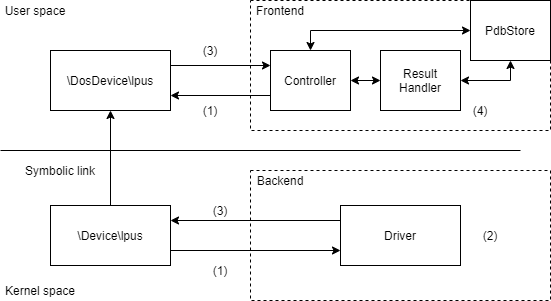
\includegraphics[scale=0.7]{images/lpus.png}
\end{figure}

% \section[Result]{Result}

We have written a few utilities to demonstrate what we can do with LPUS. The
utilities are pool tag scanning for processes, threads, drivers, files, kernel
modules; traversing the list of processes from \texttt{PsActiveProcessHead},
\texttt{KiProcessListHead}, \texttt{HandleTableListHead}; traversing the list
of loaded kernel module from \texttt{PsLoadedModuleList}; list out the unloaded
drivers, and the SSDT table; and inspecting any driver's 28 major functions.
We have also written a command similar to \texttt{psxview} of Volatility to
compare the results of processes found by many methods.

Although currently LPUS is only tested in Windows 7 and Windows 10 in
VirtualBox, it gives positive results. LPUS run and output the scanned objects
without crashing the systems. The results are checked alongside with WinDbg, a
Windows debugger, attached to the machine in virtualization. The test perform
as follows, LPUS runs and out the result, then the results are checked by
stoping the machine and attaching WinDbg. In WinDbg, commands such as
\texttt{dt} can be used to output the detail of a structure at an address, we
checked for every object found by LPUS with WinDbg. For list traversing, we
used the command in Listing.\ref{} to get the list of address in global lists.
The SSDT and driver 28 major functions is not checked through WinDbg, we
believe the addresses should be in kernel modules, which upon checking all
addresses output belongs to kernel modules. We also conducted a memory
acquisition using VirtualBox and WinPmem and compare the results found with
Volatility, the acquisition process happens seconds after the scans took place.
The results between LPUS, WinDbg and Volatility by VirtualBox memory
acquisition and Volatility by WinPmem is provided in Table.\ref{}.

% TODO: insert test result table


\chapter[Experiments]{Experiments}

The LPUS system is capable of doing many things. In this chapter, we list the
experiments that we took with LPUS and their results.

\section[Overview of what LPUS can do]{Overview of what LPUS can do}

The Windows kernel has global variables to control the system. LPUS can read
these global variables directly and collect the system information. In Section
7.2, we show how LPUS reads global variables to get the system information.
LPUS can perform pool tag scanning on both paged and non-paged pools, but
scanning with paged pool is more sophisticated as pages must be in RAM before
accessing. In Section 7.3, we show how LPUS performs pool tag scanning in the
non-paged pool region. Information collected will be further used for analysis,
especially finding hidden malware. In Section 7.4, we show how LPUS aggregates
collected information to apply malware detection.

\section[Using global variables]{Using global variables}

LPUS can get the global lists as described in Section 2.2.4, but in theory,
LPUS can access any global variables given the offset from the kernel base
address.  Many variables are not documented by Windows, to use these variables,
one must know the type and value they hold. Any individual having in-depth
knowledge in the Windows Internals will be benefited by using LPUS. In Table
\ref{tab:globalvars}, we list a few other kernel variables in Windows 7 and the
value they represent. Keep in mind that LPUS can access any kernel variable,
but a deep understanding of what the variables hold is required if we want to
use them to get the system information.

\begin{table}[t]
\centering
\begin{tabular}{ll}
\hline
  Global variable               \\ \hline
  MmPhysicalMemoryBlock         \\
  MmSystemRangeStart            \\
  MmHighestPossiblePhysicalPage \\
  MmPfnDatabase                 \\
\hline
\end{tabular}
\caption{Some kernel global variables}
\label{tab:globalvars}
\end{table}

Right now, LPUS only uses the variables that holds the pointer to lists of
process \texttt{PsActiveProcessHead}, \texttt{KiProcessListHead},
\texttt{HandleTableListHead}, the list of kernel modules
\texttt{PsLoadedModuleList}, the list of unloaded drivers
\texttt{MmUnloadedDrivers}, and the SSDT table \texttt{KiServiceTable}.  LPUS
listing the SSDT can be seen in Figure \ref{fig:ssdt_lpus}. LPUS listing the
unloaded drivers can be seen in Figure \ref{fig:unloaded_lpus}.

\begin{figure}[h]
  \centering
  \caption{LPUS lists the SSDT}
  \label{fig:ssdt_lpus}
  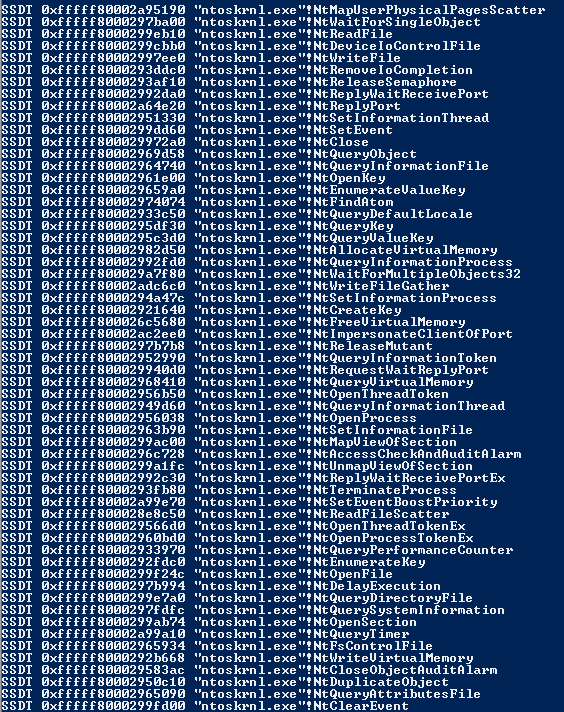
\includegraphics[scale=1]{images/ssdt_lpus.png}
\end{figure}

\begin{figure}[h]
  \centering
  \caption{LPUS lists the unloaded drivers}
  \label{fig:unloaded_lpus}
  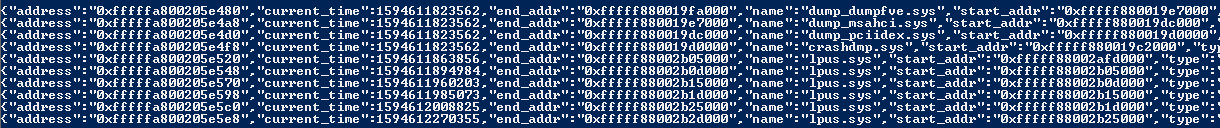
\includegraphics[scale=0.6]{images/unloaded_lpus.png}
\end{figure}

\section[Pool tag scanning]{Pool tag scanning}

LPUS supports a module to do pool tag scanning on the non-paged pool region.
Rekall on Section 3.2.3, the non-paged pool region can be accessed from the
kernel base by traversing the kernel structure as described in Table
\ref{tab:nonpaged}.  LPUS follows the table and gets the start and end of the
non-paged pool region.  The scan is performed page by page. If a page is
invalid, it is skipped. On every page, LPUS checks incrementally every
four-byte looking for the tag provided. If the tag matches, LPUS will check the
header for pool type and block size. A valid block must have the pool equal to
2 (enumeration of the non-paged pool), and the size must be larger than the
structure being found.  The search on the non-paged pool done by LPUS is
illustrated in pseudocode in Listing \ref{lst:poolscan}.

\begin{lstlisting}[language=cpp,caption={Pool Scan},label={lst:poolscan},float,floatplacement=H]
// Driver code
PVOID scan(ULONG64 startAddress, ULONG64 endAddress, ULONG tag) {
    POOL_HEADER p;
    PVOID currentAddr = (PVOID)startAddress;
    while (true) {
        if ((ULONG64)currentAddr >= endAddress)
            break;

        if (!MmIsAddressValid(currentAddr)) {
            currentAddr = (PVOID)((ULONG64)currentAddr + PAGE_SIZE);
            continue;
        }
        if (!MmIsAddressValid((PVOID)((ULONG64)currentAddr + 0x10))) {
            // >> currentAddr is at the end of a page,
            //    currentAddr+0x10 is a bad page
            //    which if we parse the header, will crash
            currentAddr = (PVOID)((ULONG64)currentAddr + 0x4);
            continue;
        }
        currentAddr = (PVOID)((ULONG64)currentAddr + 0x4);

        toPoolHeader(&p, (PVOID)currentAddr);
        if (p.poolType != 2) continue;
        if (p.tag != tag)
            continue;

        return p.addr;
    }
    return (PVOID)endAddress;
}

// User application code
// repeatedly call scan
PVOID ptr = poolStart;
while (ptr != poolEnd) {
  ptr = scan(ptr, poolEnd, tag);
  if (ptr == poolEnd) break;
  POOL_HEADER block = (POOL_HEADER*) ptr;
  if (block->PoolSize * 16 < structSize) {
    ptr += 0x4;
    continue;
  }
  // === the block is valid ===
  // parse data in block
  // ==========================
  ptr += block->PoolSize * 16;
}

\end{lstlisting}

Paged pool can also be scanned, in Windows 7 there are two variables showing
where the paged pool is, \texttt{MmPagedPoolEnd} and
\texttt{MmSizeOfPagedPoolInBytes}. \texttt{MmPagedPoolEnd} holds the end of the
paged pool and \texttt{MmSizeOfPagedPoolInBytes}. We can easily find the start
and end of the paged pool. However, scanning in this paged pool is more
complex.  The paged pool does not always reside in the physical memory, and
they will be paged out if not needed. To prevent this, we have to \textit{lock}
the page inside the memory first. This can be done by calling
\texttt{MmProbeAndLockPages}.  After locking the page, we can access the memory
as usual. There is another aspect we must pay attention to, the page validity.
This paged pool range is vast, many pages may not be valid and will trigger
exception on access. In theory, the paged pool can be scanned, but we have not
implemented the feature.  One big reason why we chose not to implement this
feature is that most important Windows objects allocation are located inside
the non-paged pool, there is no reason to scan the paged pool if the
information found is limited or none.

The LPUS module implementing pool tag scanning returns the block address on any
block matches the criteria. For ordinary objects without headers, by skipping
the \texttt{\_POOL\_HEADER}, we get the address to the object. For executive
objects, which have headers around them, it is harder to get the object's
address. We currently check the member fields for validity, e.g., for
\texttt{\_EPROCESS} and \texttt{\_ETHREAD}, we check the \texttt{CreateTime} to
be between the OS boot time and scan time. We have implemented pool tag
scanning for \texttt{\_EPROCESS}, \texttt{\_ETHREAD},
\texttt{\_DRIVER\_OBJECT}, \texttt{\_LDR\_DATA\_TABLE\_ENTRY},
\texttt{\_FILE\_OBJECT}. LPUS can also scan objects related to internet
connections, kernel callbacks, and mutexes, but we have difficulty implementing
these objects and leaving them for future development.

The results of pool tag scanning for \texttt{\_EPROCESS} and \texttt{\_ETHREAD}
can be seen in Figure \ref{fig:psxview}, where we demonstrate LPUS comparing
the processes found by list walking and scanning.

\begin{figure}[h]
  \centering
  \caption{LPUS compare lists of process}
  \label{fig:psxview}
  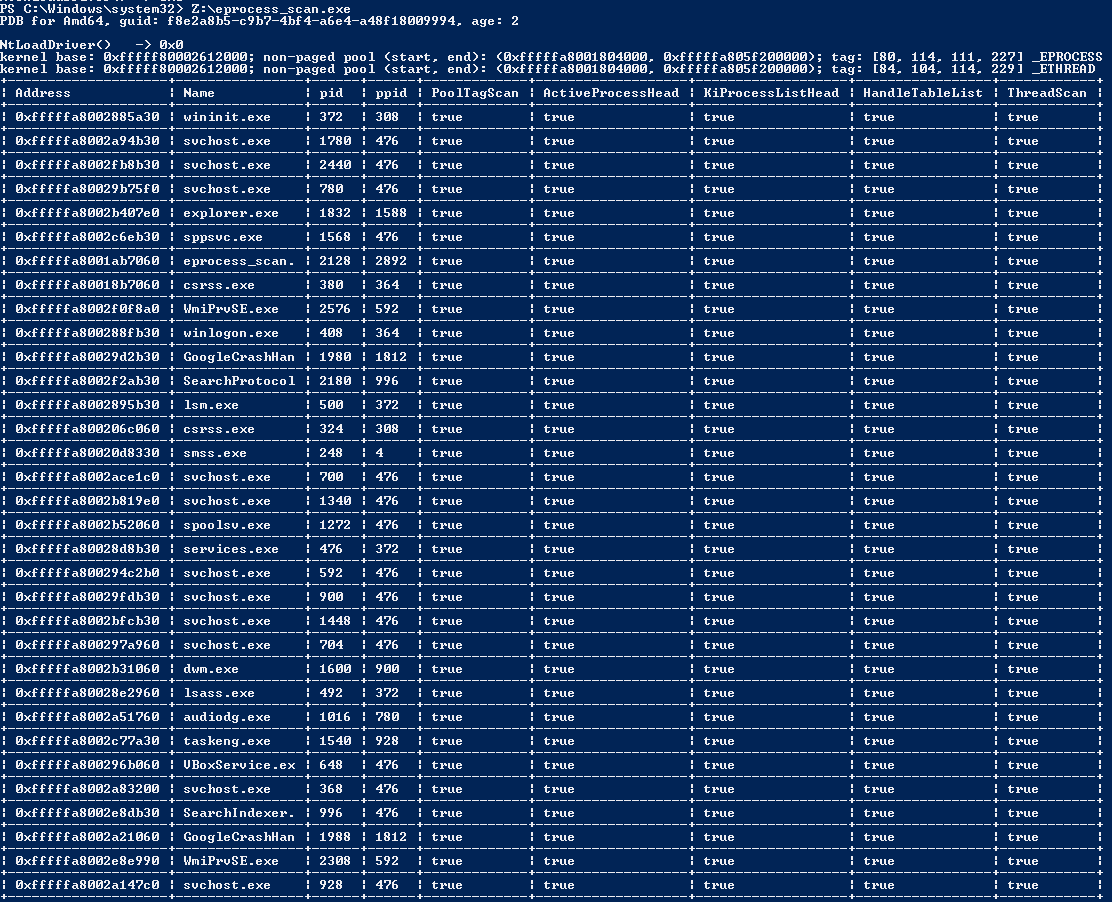
\includegraphics[scale=0.7]{images/psxview.png}
\end{figure}

\section[Driver's IRP listing]{Driver's IRP listing}

LPUS supports IRP hooking detection by inspecting the driver list
\texttt{MajorFunction}. To do this, LPUS will first scan for
\texttt{\_DRIVER\_OBJECT} and \texttt{\_LDR\_DATA\_TABLE\_ENTRY} and saves the
results into two list, drivers and modules. When the user chose a driver to
inspect the \texttt{MajorFunction}, LPUS will loop through each function
pointer in the \texttt{MajorFunction} list and search for the module containing
the function. Figure \ref{fig:irp_lpus} is the sample results of LPUS when
inspecting a driver object at a specific address.

\begin{figure}[h]
  \centering
  \caption{LPUS inspects the IRP of a driver}
  \label{fig:irp_lpus}
  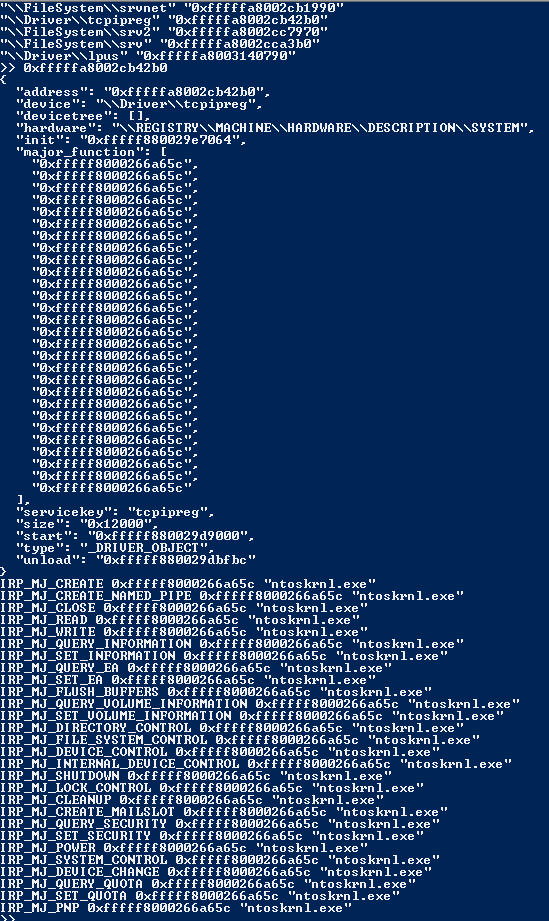
\includegraphics[scale=1]{images/irp_lpus.png}
\end{figure}

% Compared to using WinDbg
% where the machine has to be stoped LPUS is a better option. WinDbg supports
% live mode by loading a special kernel driver when the system loads and requires
% the user to enable debug mode, LPUS can work without these requirements and can
% still query the kernel system.

\section[Comparing LPUS]{Comparing LPUS}

In this section, we compare LPUS with Volatility. We set up the test
environment as follows. Run an instance of Windows 7 SP1 64-bit in Virtual Box.
Connect WinDbg to debug the OS. Run LPUS and output the results into a JSON
file.  Immediately after LPUS terminates, pause the system with WinDbg. In
WinDbg use the \texttt{.dump /f} command to generate a full kernel dump, full
RAM contents. After WinDbg finishes, use \texttt{VBoxManage}, a utility to
manage machine instances in Virtual Box, to output the RAM content. With the
two memory files, one from WinDbg and one from Virtual Box, we run Volatility
commands to get the same information as LPUS. We then use a Python script to
compare LPUS output with the Volatility results using the WinDbg memory file,
and Volatility results using the Virtual Box memory file. The results are
compared using the object's addresses. In Table \ref{testinfo}, we list the
information to compare on the Volatility command to get the information. In
Table \ref{testresult}, we have the results of the comparison.


\begin{table}[t]
\centering
\begin{tabular}{ll}
\hline
  Information         & Volatility command \\ \hline
  Process list        & pslist             \\
  Process scan        & psscan             \\
  Threads             & threads            \\
  Thread scan         & thrdscan           \\
  Kernel modules      & modscan            \\
  Kernel module scan  & modscan            \\
  Drivers             & driverscan         \\
  Unloaded drivers    & unloadedmodules    \\
  SSDT                & ssdt               \\
\hline
\end{tabular}
\caption{Test information and Volatility command}
\label{tab:testinfo}
\end{table}


\begin{table}[t]
\centering
\begin{tabular}{lrrrr}
command         & common & LPUS only & WinDbg only & VBox only \\
\hline
driverscan      & 105    & 2         & 1           & 1         \\
modscan         & 67     & 0         & 71          & 71        \\
modules         & 137    & 1         & 0           & 0         \\
pslist          & 39     & 1         & 0           & 0         \\
psscan          & 0      & 41        & 0           & 0         \\
thrdscan        & 0      & 41        & 0           & 0         \\
threads         & 574    & 16        & 4           & 23        \\
unloadedmodules & 4      & 0         & 1           & 1         \\
ssdt            & 390    & 11        & 836         & 836       \\
\hline
\end{tabular}
\caption{Test results}
\label{tab:testresult}
\end{table}

\chapter[Discussion]{Discussion}

Every solution has its advantages and disadvantages. LPUS is no exception. In
this chapter we discuss the advantages LPUS has over other tools and also
criticize the disadvantages of LPUS.

\section[Advantages]{Advantages}

As of the prerequisites, LPUS only needs to be run as an Administrator on an
internet-connected machine to perform forensics on the current machine. LPUS
can works on any Windows version higher than 7 and easily supports new version.

As of the results, LPUS can give the same result to Volatility if the memory
file is taken after LPUS finishes. But because LPUS can perform live forensics,
we expect LPUS to fetch new result time by time.

LPUS works without the installation of any third-party plugins. Everything is
compiled into a binary and a driver. The Visual C++ module is also statically
compiled, so LPUS can be used on any Windows machine without installing
anything.

LPUS directly queries the kernel data without having a memory file. LPUS gets
the kernel base address and traverses through the kernel space without crashing
the system.

LPUS can apply forensics techniques to help one finds the hidden process and
much more information. This thesis's scope is about finding hidden process
memory, but we can see that LPUS can do more than just that. LPUS can apply
more forensics methods and develop a whole set of functionalities that
Volatility or Rekall has.

\section[Disadvantages]{Disadvantages}

LPUS backend does not check for address validity when fetching bytes from the
kernel, which will crash the system if an invalid address is asked. LPUS should
check if the address is in the kernel space and must ensure the page containing
the address is in memory. LPUS backend is copying the whole memory (from
address and of \texttt{size} bytes) into the buffer without splitting into many
copy operations.  If the front end asks the backend a big memory space
containing some invalid memory holes, the system crashes.

LPUS is using members in the structure to find the address of an object when
doing pool tag scanning, this would give false result if malware rewrite these
fields.  LPUS could check for optional headers for executive objects. Or
better, LPUS can use other scientific methods to answer the question, ``Is the
structure reside in this byte-array''.

LPUS can not access the user-space address and misses useful information.
Further research is needed to access the process user-space to perform
forensics.

LPUS backend does not check if the process asking is the LPUS frontend. A
program can imitate LPUS frontend and access the kernel. Both the back end and
the front end must have a protocol to verify each other to prevent application
access to the kernel space.

\section[Other minor problems]{Other minor problems}

LPUS has some design issues that can be fixed to make LPUS better. These are
not severe problems but worth mentioning.

The kernel driver has to be installed inside the \texttt{C:\textbackslash
\textbackslash Windows\textbackslash System32 \textbackslash drivers} while it
is possible to put the driver anywhere to load.

LPUS downloads the debug symbols for the systems, and this requires an internet
connection. We can download the debug symbols for every system and pack it in
the LPUS distribution and use a pre-downloaded PDB file.

Loading the kernel driver is using the undocumented API \texttt{NtLoadDriver},
while most programs loading the driver uses \textit{Services} feature in
Windows.

LPUS is now distributed as multiple binaries. We need to rework them into one
binary and use CLI arguments to select forensics methods.


\chapter[Conclusion]{Conclusion}

\section[Overall result]{Overall result}

During the studies and work on the thesis topic, ``Finding hidden processes in
a running machine'', we have gained knowledge on using forensics methods to
detect hidden processes. Not only that, but we have also implemented a
prototype, LPUS system, to perform forensics without using the memory file and
running live. The first tests with LPUS show positive results in Windows 7 and
Windows 10.

\section[Future works]{Future works}

LPUS is at its final stage for the thesis outcome. The results are still
printed out to the console. We hope to have a Graphical User Interface, GUI,
and display information in a more comprehensible way. LPUS is still having many
issues, big and small. These issues have to be fixed to provide a more stable
experience.

The current status of LPUS performs a few forensics methods, yet we can
implement more forensics methods and make LPUS a competitive tool alongside
with Volatility and Process Explorer. To do this, extensive research into the
Windows Internal and malware analysis are needed.  LPUS can be extended to make
a shell, like VolShell or Rekall interactive shell, where users can program to
perform automatic analysis.


% \include{ketluan}                           %%% có thể thay đổi
% \include{chdanhmuccongbo}                   %%% có thể thay đổi

\nocite{*}
\VKngatTrang                                %%% ngắt trang để chuyển sang tài liệu tham khảo
\VKtaiLieuThamKhao                          %%% tài liệu tham khảo
% \VKdanhSoPhuLuc                             %%% bắt đầu đánh số cho phụ lục

% \include{phuluccaidat}                      %%% có thể thay đổi

\end{document}

